%% LaTeX2e class for student theses
%% sections/evaluation.tex
%% 
%% Karlsruhe Institute of Technology
%% Institute for Program Structures and Data Organization
%% Chair for Software Design and Quality (SDQ)
%%
%% Dr.-Ing. Erik Burger
%% burger@kit.edu
%%
%% Version 1.3.6, 2022-09-28

\chapter{Evaluation}
\label{ch:Evaluation}

In the following chapter we will evaluate the experiments we conducted. We start off by explaining our evaluation metrics, both for Continual Active Learning
and when applying Continual Active Learning to Model Stealing. Afterwards we will present the results of our experiments and discuss the findings.

\section{Evaluation Metrics}
\label{sec:Evaluation:Metrics}
% Describe that we used agreement for model stealing (and on which dataset) and 
% validation accuracy for the model stealing experiments. and hyperparameters

\subsection{Metrics for Continual Active Learning}
\label{sec:Evaluation:Metrics:CAL}
When choosing a metric to evaluate Continual Active Learning, we need to remember the motivation of the approach. We proposed the Continual Active Learning approach
mainly to reduce the mainly to mitigate the overhead of pure Active Learning compared to the classic training loop. Therefore, it is desirable to incorporate a metric
which measures this goal. In our case, this is the overall execution time. However, execution time is not the only metric we want to use to evaluate the approach. Since 
the second goal of the Continual Learning approach is to improve model performance, we will also evaluate the experiments based on this. What a makes a machine learning 
model performant has been discussed vividly in the literature. In our case, we will use the validation accuracy as a metric to evaluate the performance of the model. It is
important to consider \textit{both} runtime and validation accuracy when evaluating the experiments. A model with low runtime and low validation accuracy is not desirable,
but neither is a model with high runtime and high validation accuracy. Since we are trying to improve Active Learning by introducing Continual Learning into the pool-based 
Active Learning process, we aim to outperform the classic pool-based Active Learning approach. More precisely, we want to reduce the runtime and increase the validation
accuracy. The success of our Continual Active Learning approach will be evaluated against the classic pool-based Active Learning approach based on the runtime improvement
and the accuracy improvement. 


\subsection{Metrics for Continual Active Learning for Model Stealing}
\label{sec:Evaluation:Metrics:CALMS}
As presented in section \ref{sec:ModelStealing:Attacks}, Model Stealing Attacks can be performed for a variety of reasons. As we build our framework on ActiveThief, we also
adopt the metrics used in the original paper. The ActiveThief framework aims purely at stealing the functionality of the model, i.e. approximation the model's relationship
between input and output best, and so does ours. Therefore, we will use the same evaluation metric, which in our case is the agreement between substitute and target model,
computed on the validation split of the target model dataset. The baseline which we compare our results against is the ActiveThief framework. We will therefore measure the 
success of using Continual Active Learning for Model Stealing by comparing the model agreement of our approach to the model agreement of the ActiveThief framework.

\section{Results}
\label{sec:Evaluation:Results}
In this section we will present the results of our experiments. As mentioned before, our experiments are split into two parts. The first part is the evaluation of our novel
Continual Active Learning Approach and the second part is evaluating the performance our the Continual Active Learning approach when applied to Model Stealing. In each of these
respective subsections we will first describe the experiments schedule for each part and then present the results of the experiments.

\subsection{Results for Continual Active Learning}
\label{sec:Evaluation:Results:CAL}
In this subsection we will first present the results of running all combinations of the Active Learning strategies BALD,Badge,CoreSet,LC and Random with the Continual Learning strategies
Naive, EWC, MAS, Alasso and IMM. Afterwards, we will analyze the behavior of a hybrid approach between Active Learning and Continual Active Learning, where we first run a few cycles with
pure Active Learning before switching to Continual Active Learning. We further analyze the performance of different strategies to initialize the labeled pool. Next, we experiment with VAAL
and AGEM.

\subsubsection{AL and Cl combinations}
\label{sec:Evaluation:Results:CAL:ALCL}
To evaluate the combination of the Active Learning strategies BALD,Badge,Coreset,LC and Random with the Continual Learning strategies Naive, EWC, MAS, Alasso and IMM, we run each combination
using a batch size of 1000,2000 and 4000. We use the CIFAR-10 dataset and the Neural Network Architecture Resnet18 for these experiments. We present the validation accuracy with increasing
size of the labeled pool as well as the overall runtime of each experiment. \par
In figure \ref{fig:Evaluation:Results:CAL:Random1000} we present the results of running the Active Learning strategy Random with the Continual Learning strategies Naive, EWC, MAS, Alasso and IMM
as well as the baseline of running pure Active Learning. We use a batch size of 1000 for these experiments. In terms of runtime, all strategies are significantly faster than the classic Active
 Learning approach. However, there is a notable gap in validation accuracy between Active Learning and all Continual
Active Learning strategies. IMM is the only Continual Learning strategy to outperform the Naive approach. EWC performs slightly worse than the Naive approach while MAS and Alasso
perform significantly worse.

\begin{figure}[ht]
    \centering
    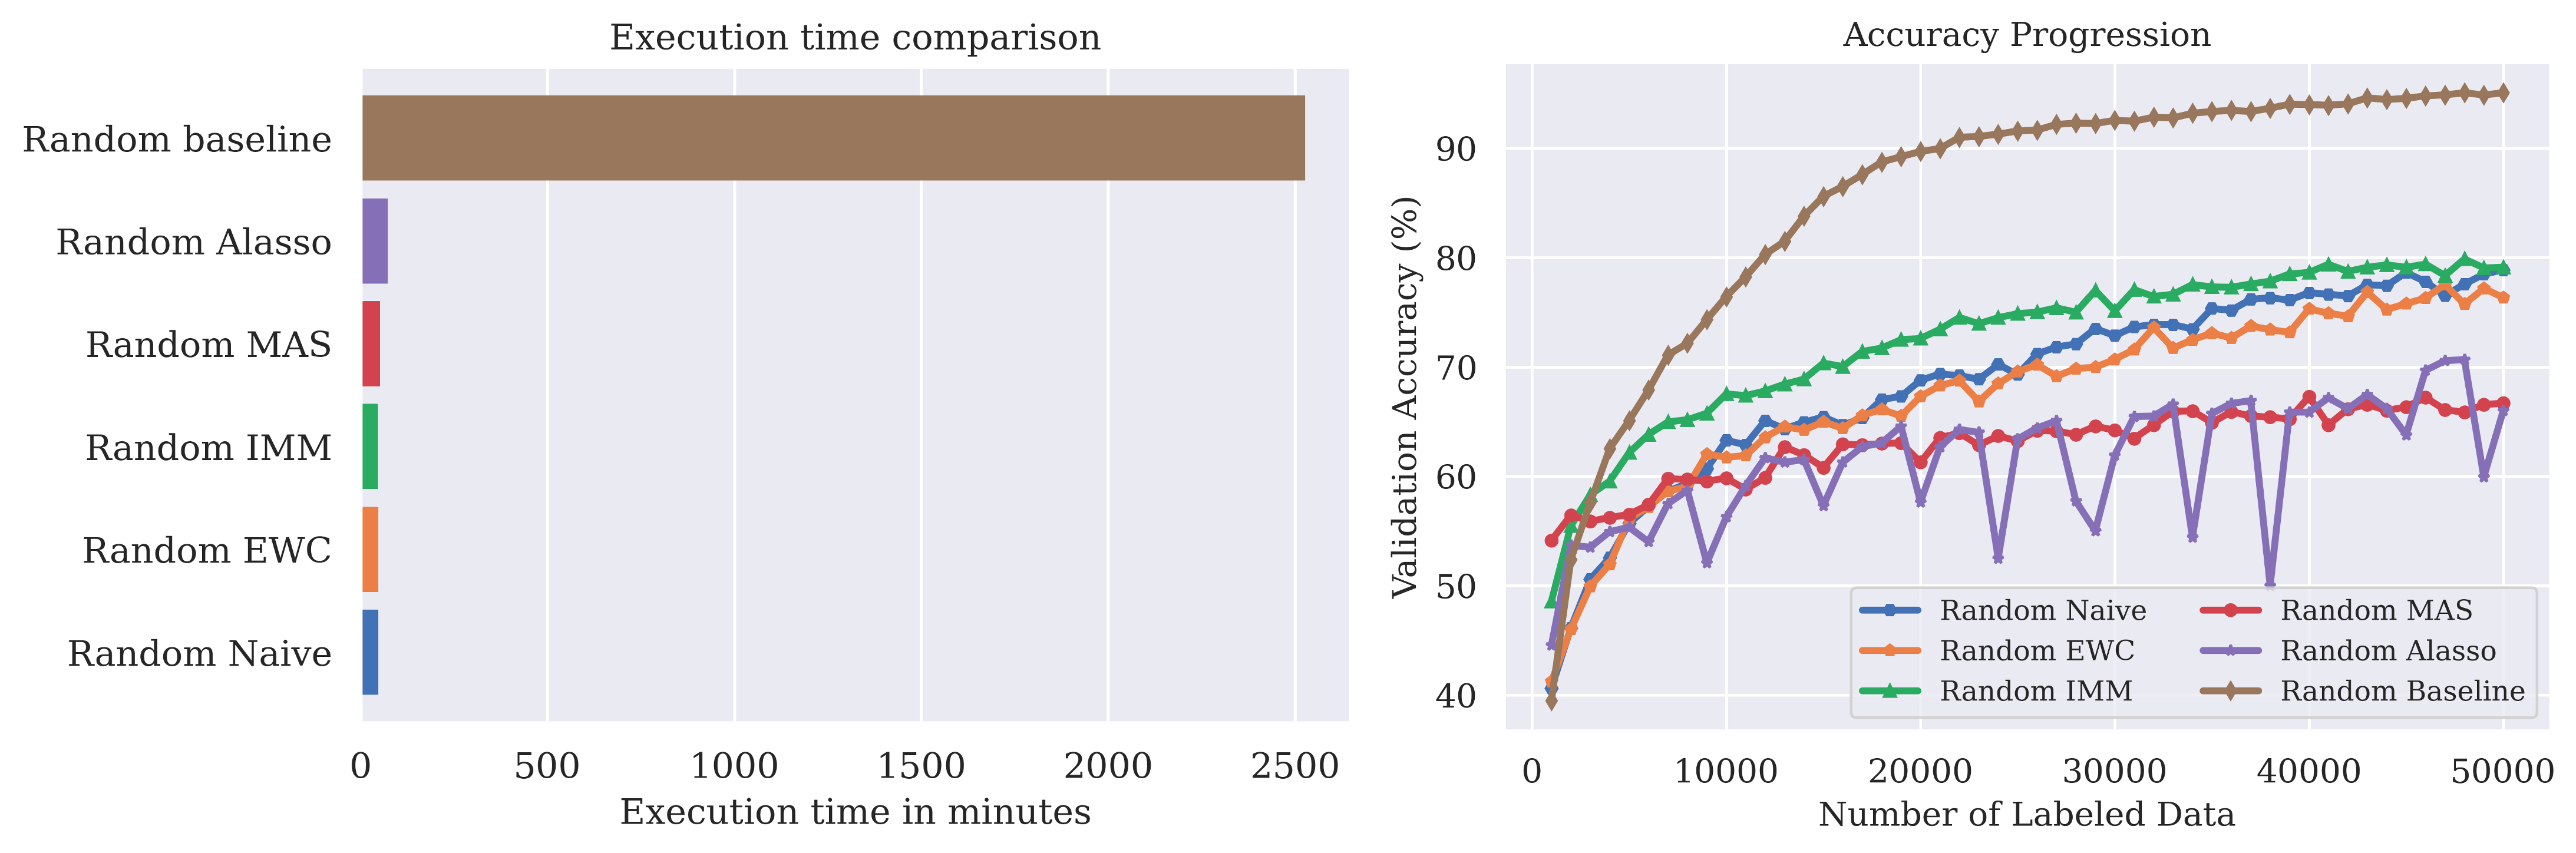
\includegraphics[width=\linewidth]{images/results_CAL/Random_CAL_1000b.png}
    \caption[Continual Active Learning Random 1000 batch size]{Comparison of Continual Learning strategies used with the Active Learning strategy random. We use a batch size of 1000 for the experiments.
    }
    \label{fig:Evaluation:Results:CAL:Random1000}
\end{figure}

\begin{figure} [ht]
    \centering
    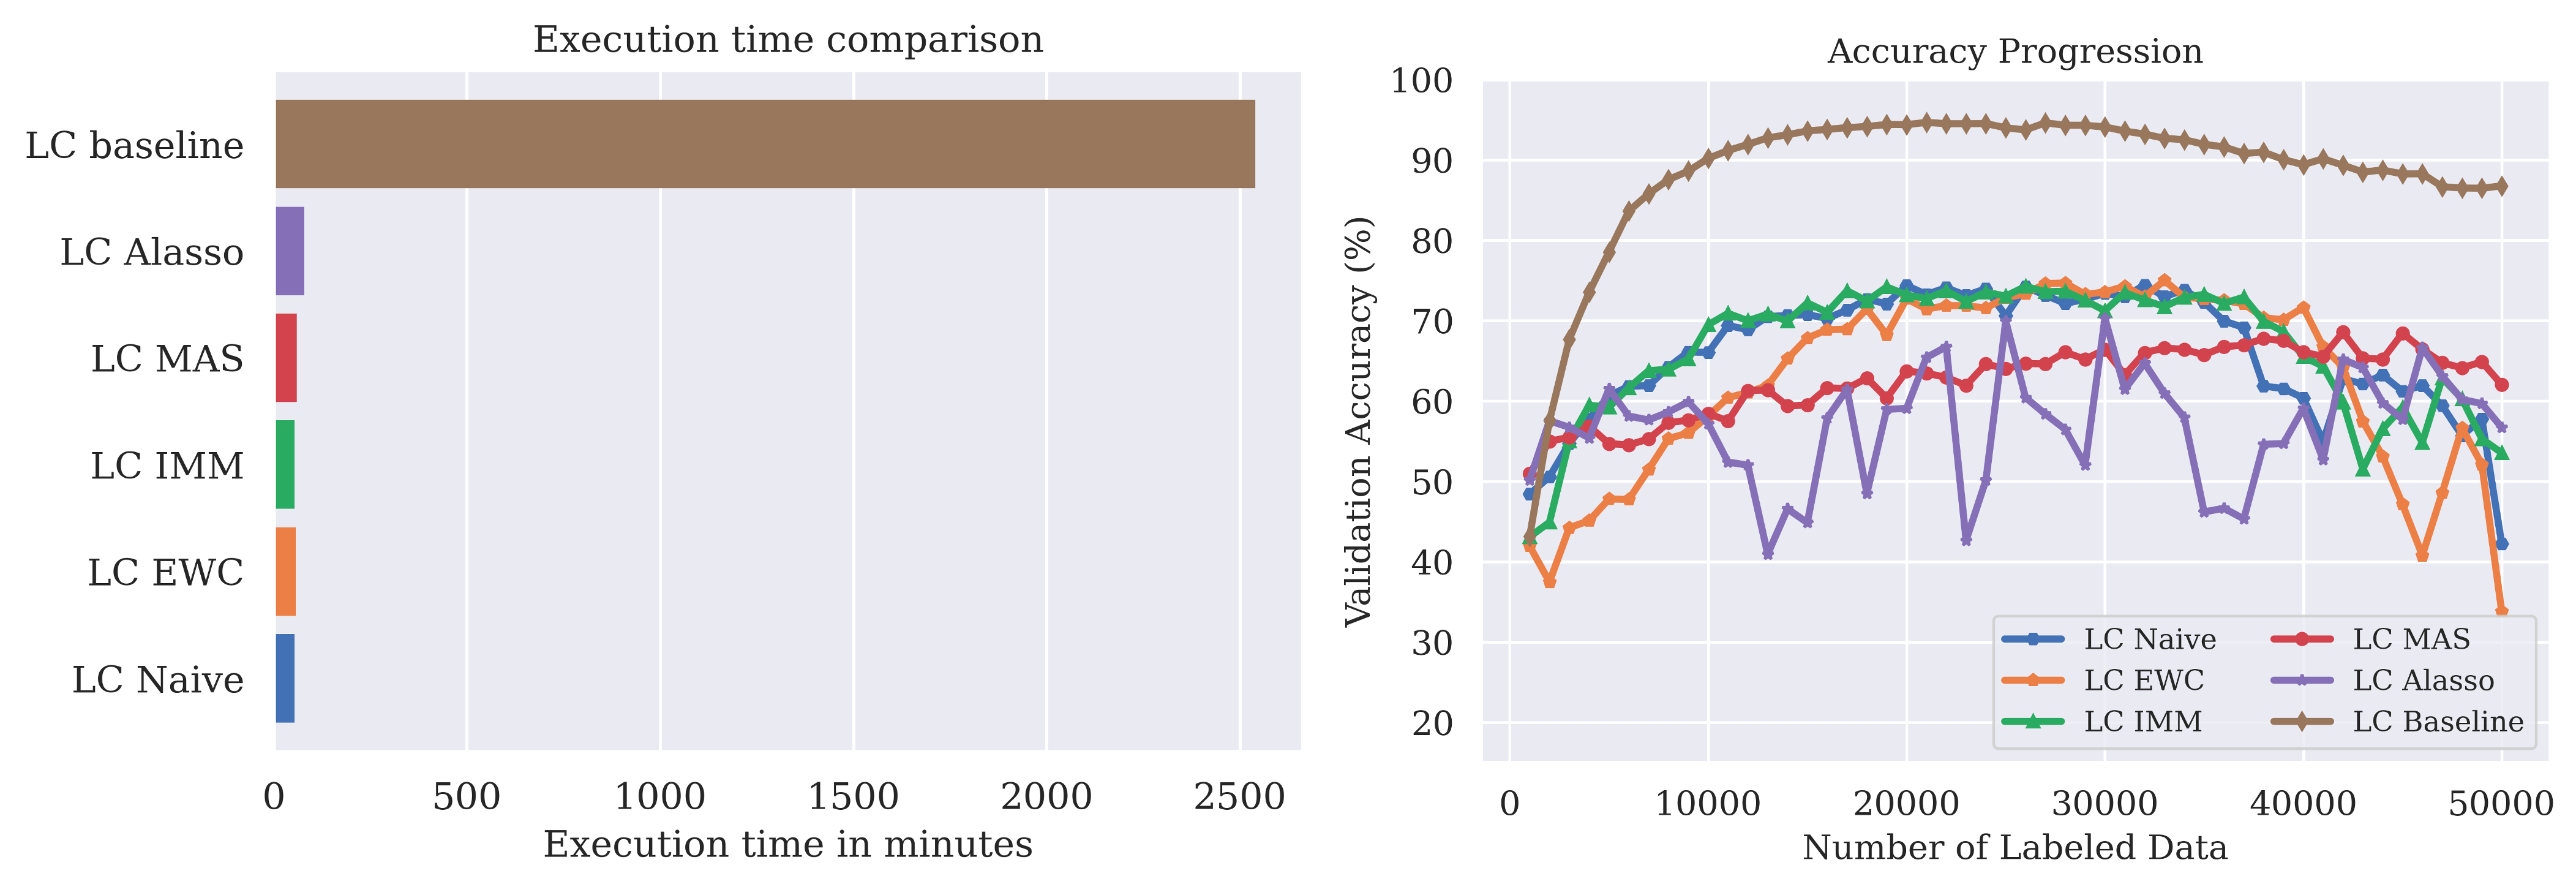
\includegraphics[width=\linewidth]{images/results_CAL/LC_CAL_1000b.png}
    \caption[Continual Active Learning Random 1000 batch size]{Comparison of Continual Learning strategies used with the Active Learning strategy LC. In terms of runtime, all
    strategies are significantly faster than the classic Active Learning approach. However, there is a notable gap in validation accuracy between Active Learning and all Continual
    Active Learning strategies. IMM and Naive perform almost identically. EWC performs slightly worse than IMM and Naive wheres MAS and Alasso perform significantly worse. Interestingly
    though, MAS performs best in the end and is the only Continual Learning strategy not to experience a  drop in accuracy whithin the final 5000 samples.}
    \label{fig:Evaluation:Results:CAL:LC1000}
\end{figure}

\begin{figure} [ht]
    \centering
    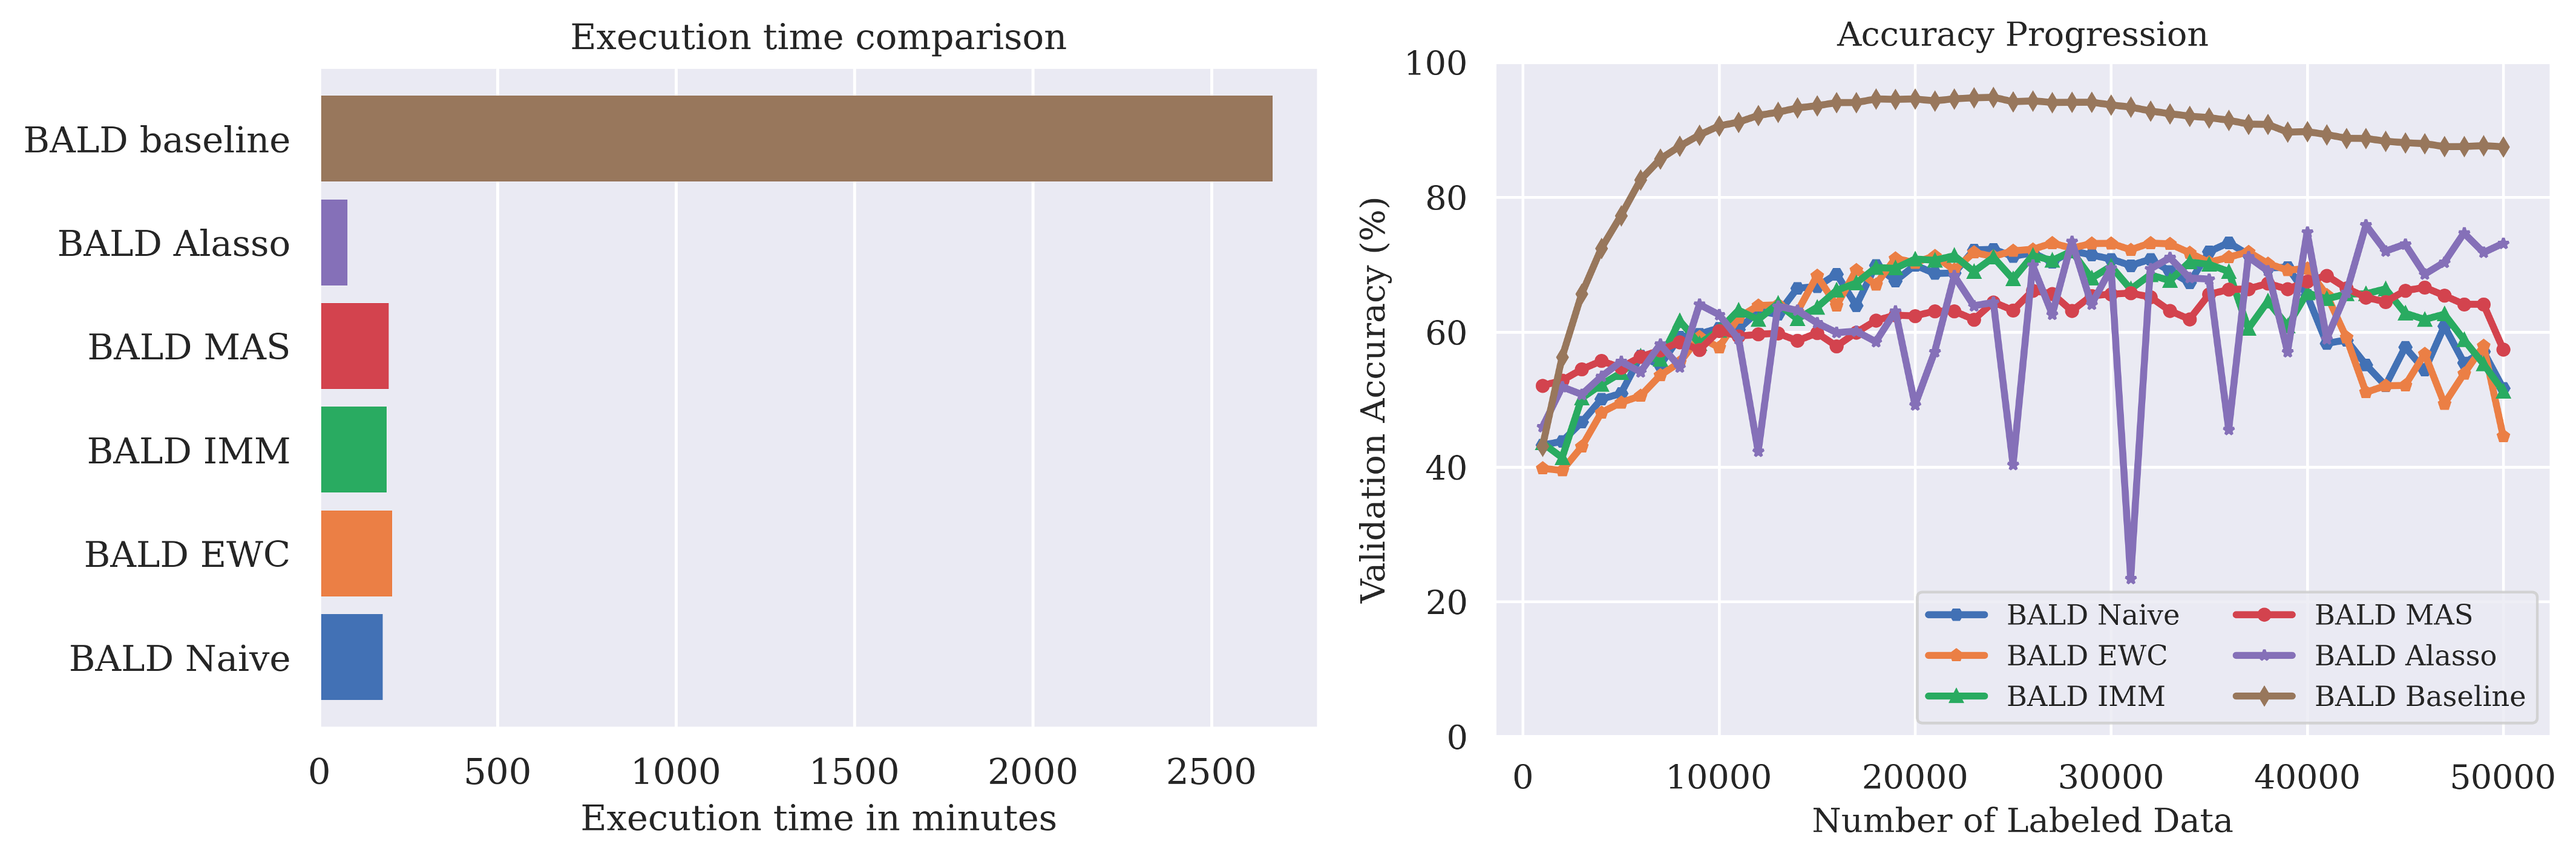
\includegraphics[width=\linewidth]{images/results_CAL/Bald_CAL_1000b.png}
    \caption[Continual Active Learning BALD 1000 batch size]{TODO: Redo BALD Plot}
    \label{fig:Evaluation:Results:CAL:BALD1000}
\end{figure}

\begin{figure} [ht]
    \centering
    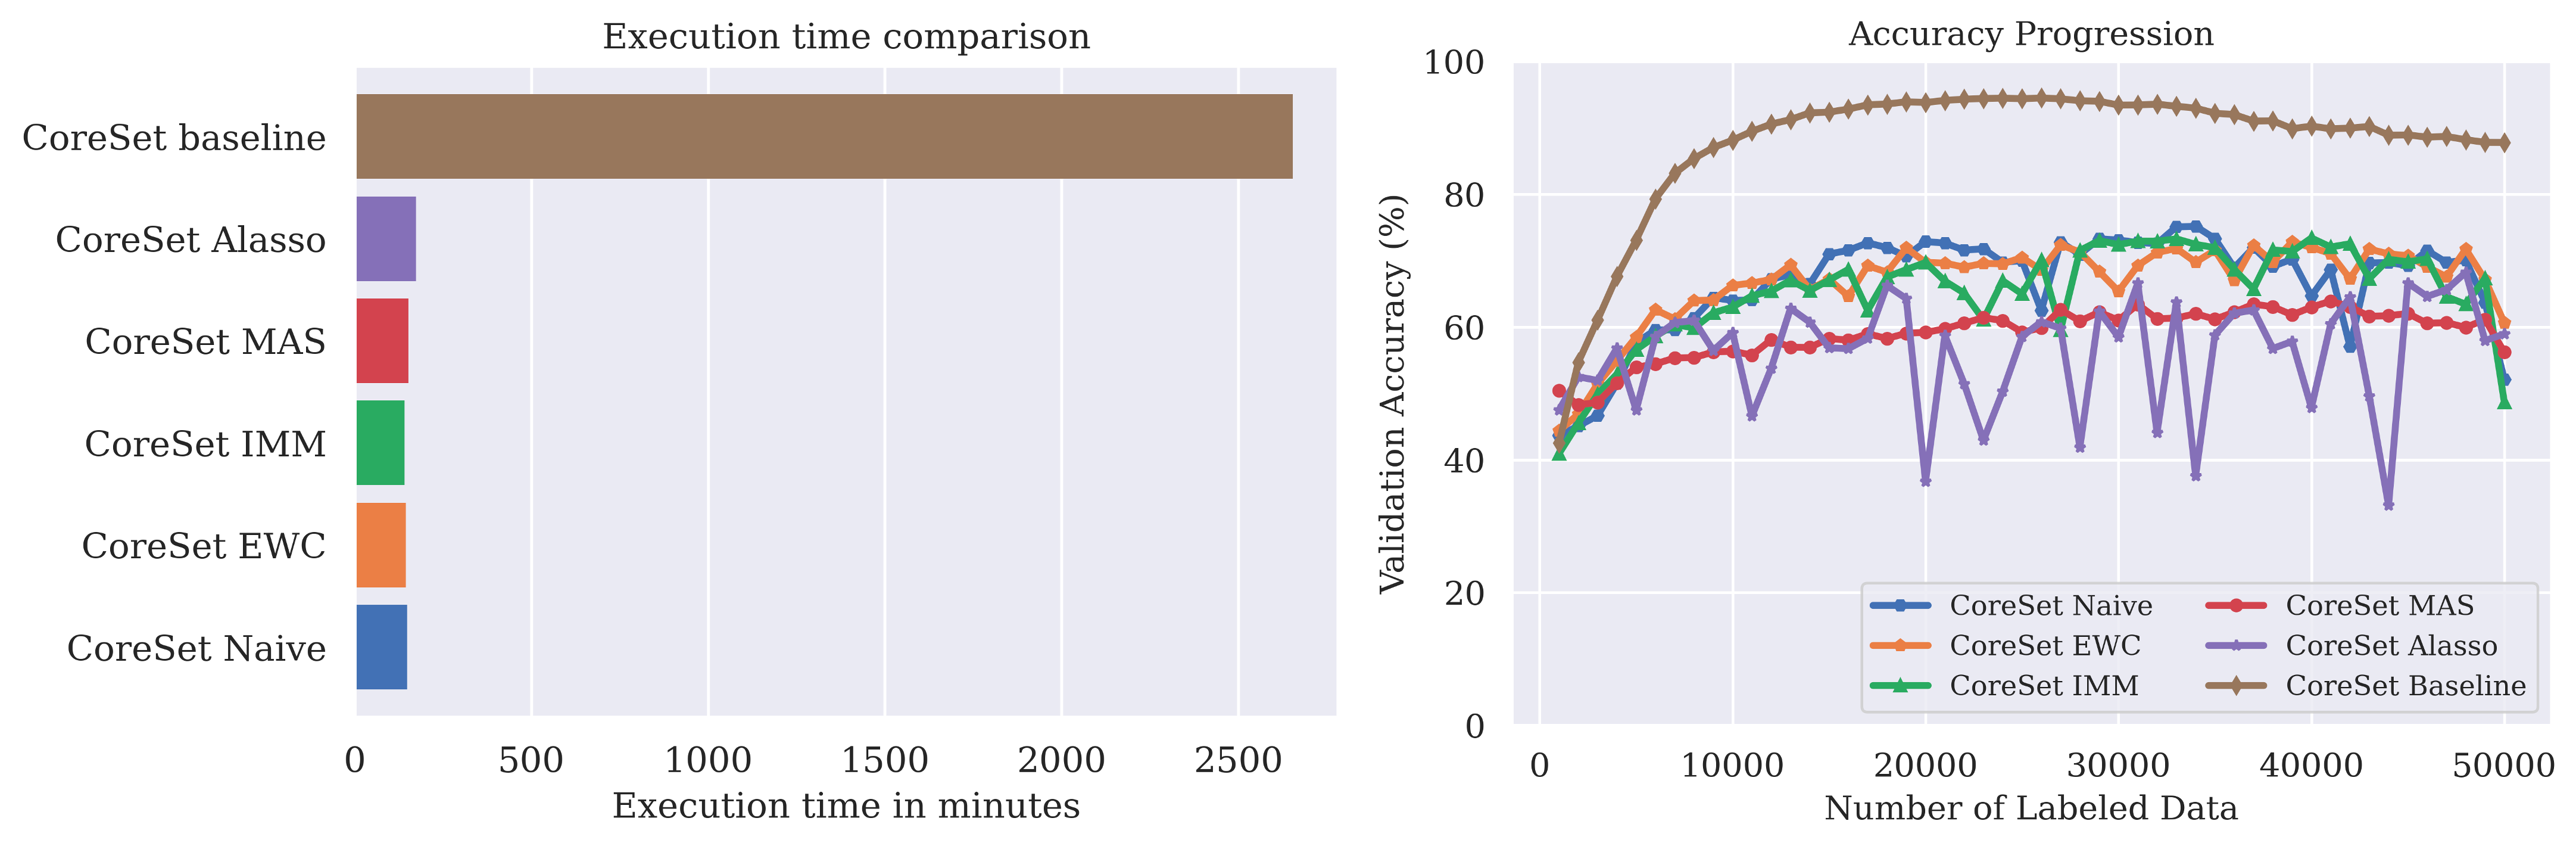
\includegraphics[width=\linewidth]{images/results_CAL/CoreSet_CAL_1000b.png}
    \caption[Continual Active Learning CoreSet 1000 batch size]{Comparison of Continual Learning strategies used with the Active Learning strategy CoreSet. In terms of runtime, all
    strategies are significantly faster than the classic Active Learning approach. However, there is a notable gap in validation accuracy between Active Learning and all Continual
    Active Learning strategies. IMM, EWC Naive perform almost similarly while MAS and Alasso fall behind.}
    \label{fig:Evaluation:Results:CAL:CoreSet1000}
\end{figure}

\begin{figure} [ht]
    \centering
    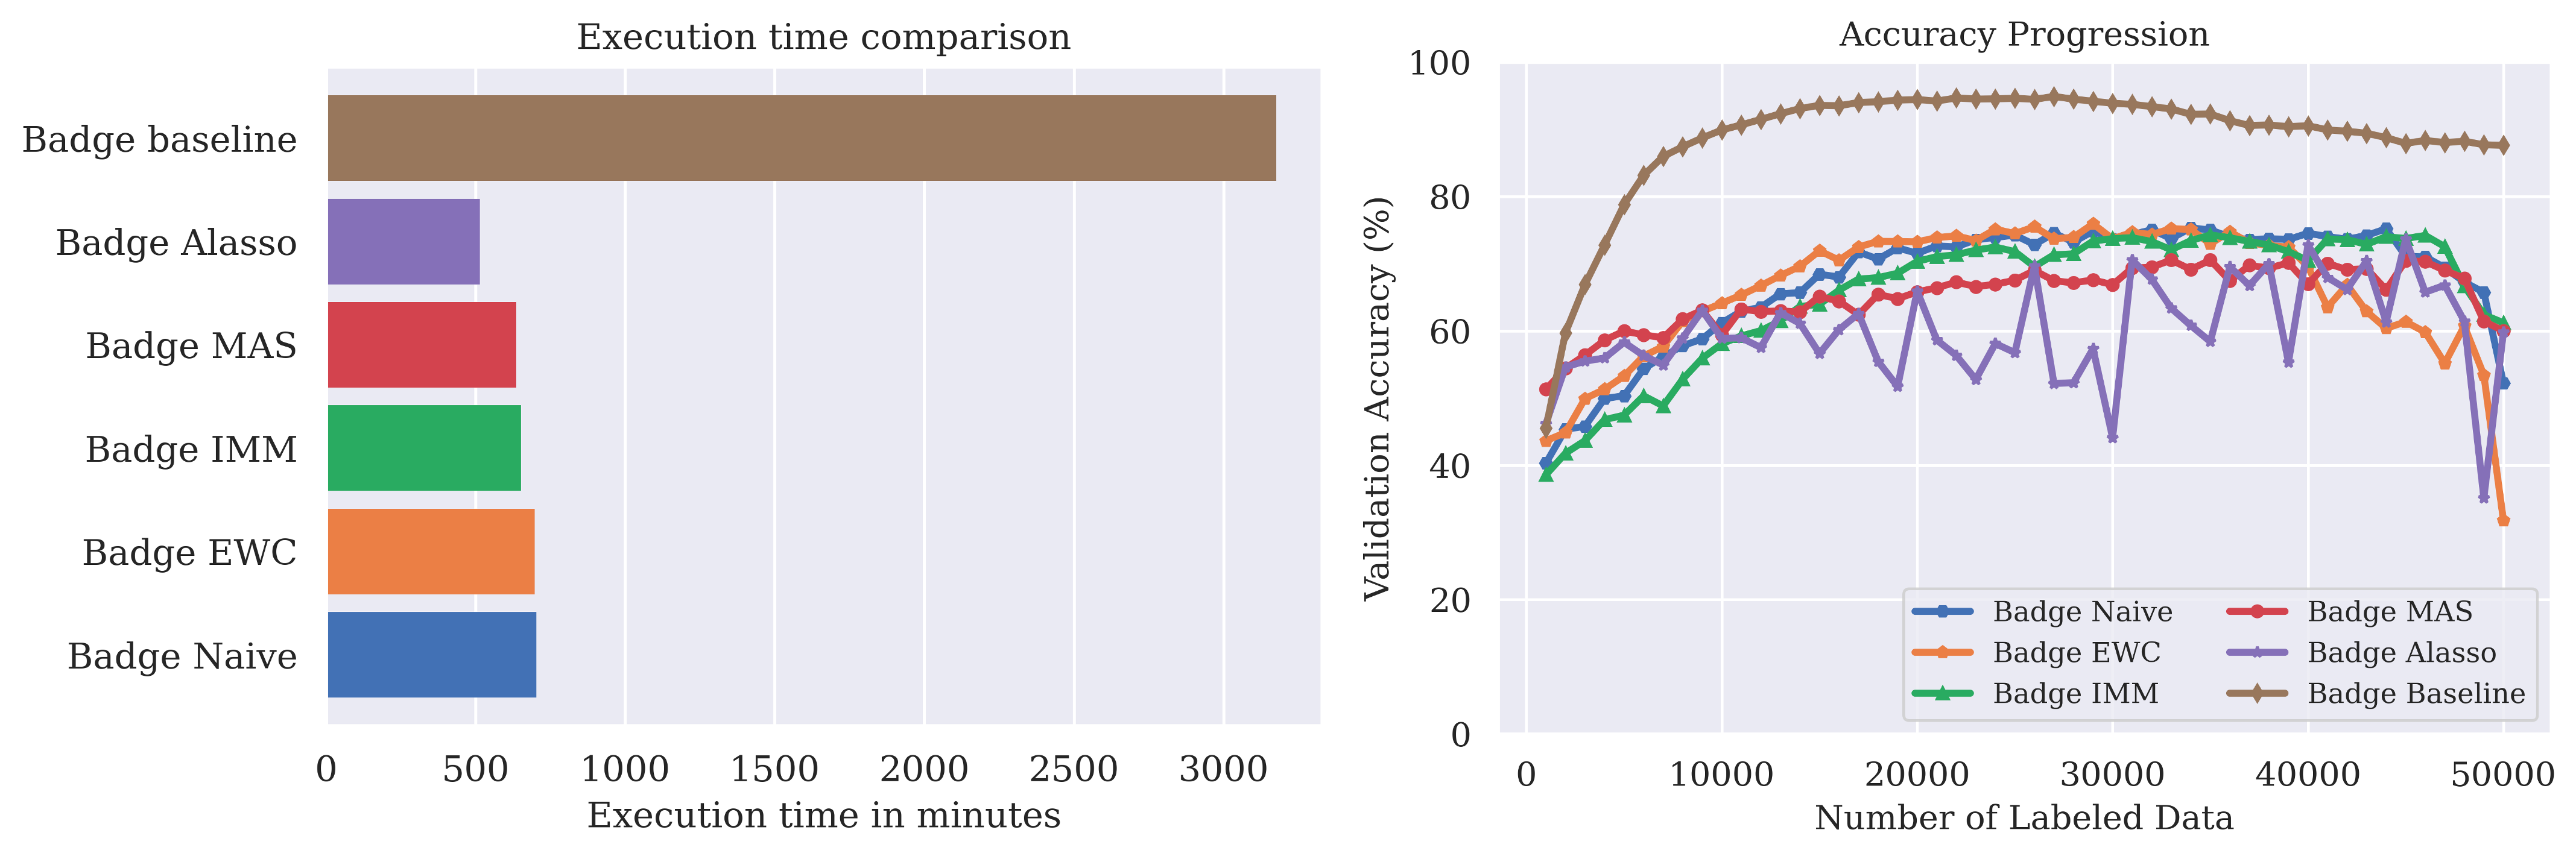
\includegraphics[width=\linewidth]{images/results_CAL/Badge_CAL_1000b.png}
    \caption[Continual Active Learning Badge 1000 batch size]{Comparison of Continual Learning strategies used with the Active Learning strategy Badge. In terms of runtime, all
    strategies are significantly faster than the classic Active Learning approach. However, there is a notable gap in validation accuracy between Active Learning and all Continual
    Active Learning strategies. EWC performs best for the first 30000 samples but falls behind in the end. IMM performs closer to Naive with an increasing amount of samples. MAS and
    Alasso perform significantly worse than the other strategies.}
    \label{fig:Evaluation:Results:CAL:Badge1000}
\end{figure}




\begin{figure} [ht]
    \centering
    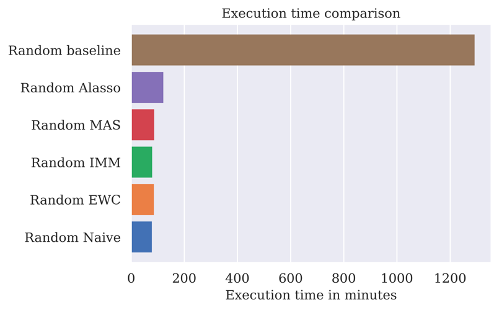
\includegraphics[width=\linewidth]{images/results_CAL/Random_CAL_2000b.png}
    \caption[Continual Active Learning Random 2000 batch size]{Comparison of Continual Learning strategies used with the Active Learning strategy Random. In terms of runtime, all
    strategies are significantly faster than the classic Active Learning approach. However, there is a notable gap in validation accuracy between Active Learning and all Continual
    Active Learning strategies. EWC performs best overall, followed closely by the Naive approach. IMM, Alasso and MAS overall perform similarly, leaving a gap towards the first 
    two strategies.}
    \label{fig:Evaluation:Results:CAL:Random2000}
\end{figure}

\begin{figure} [ht]
    \centering
    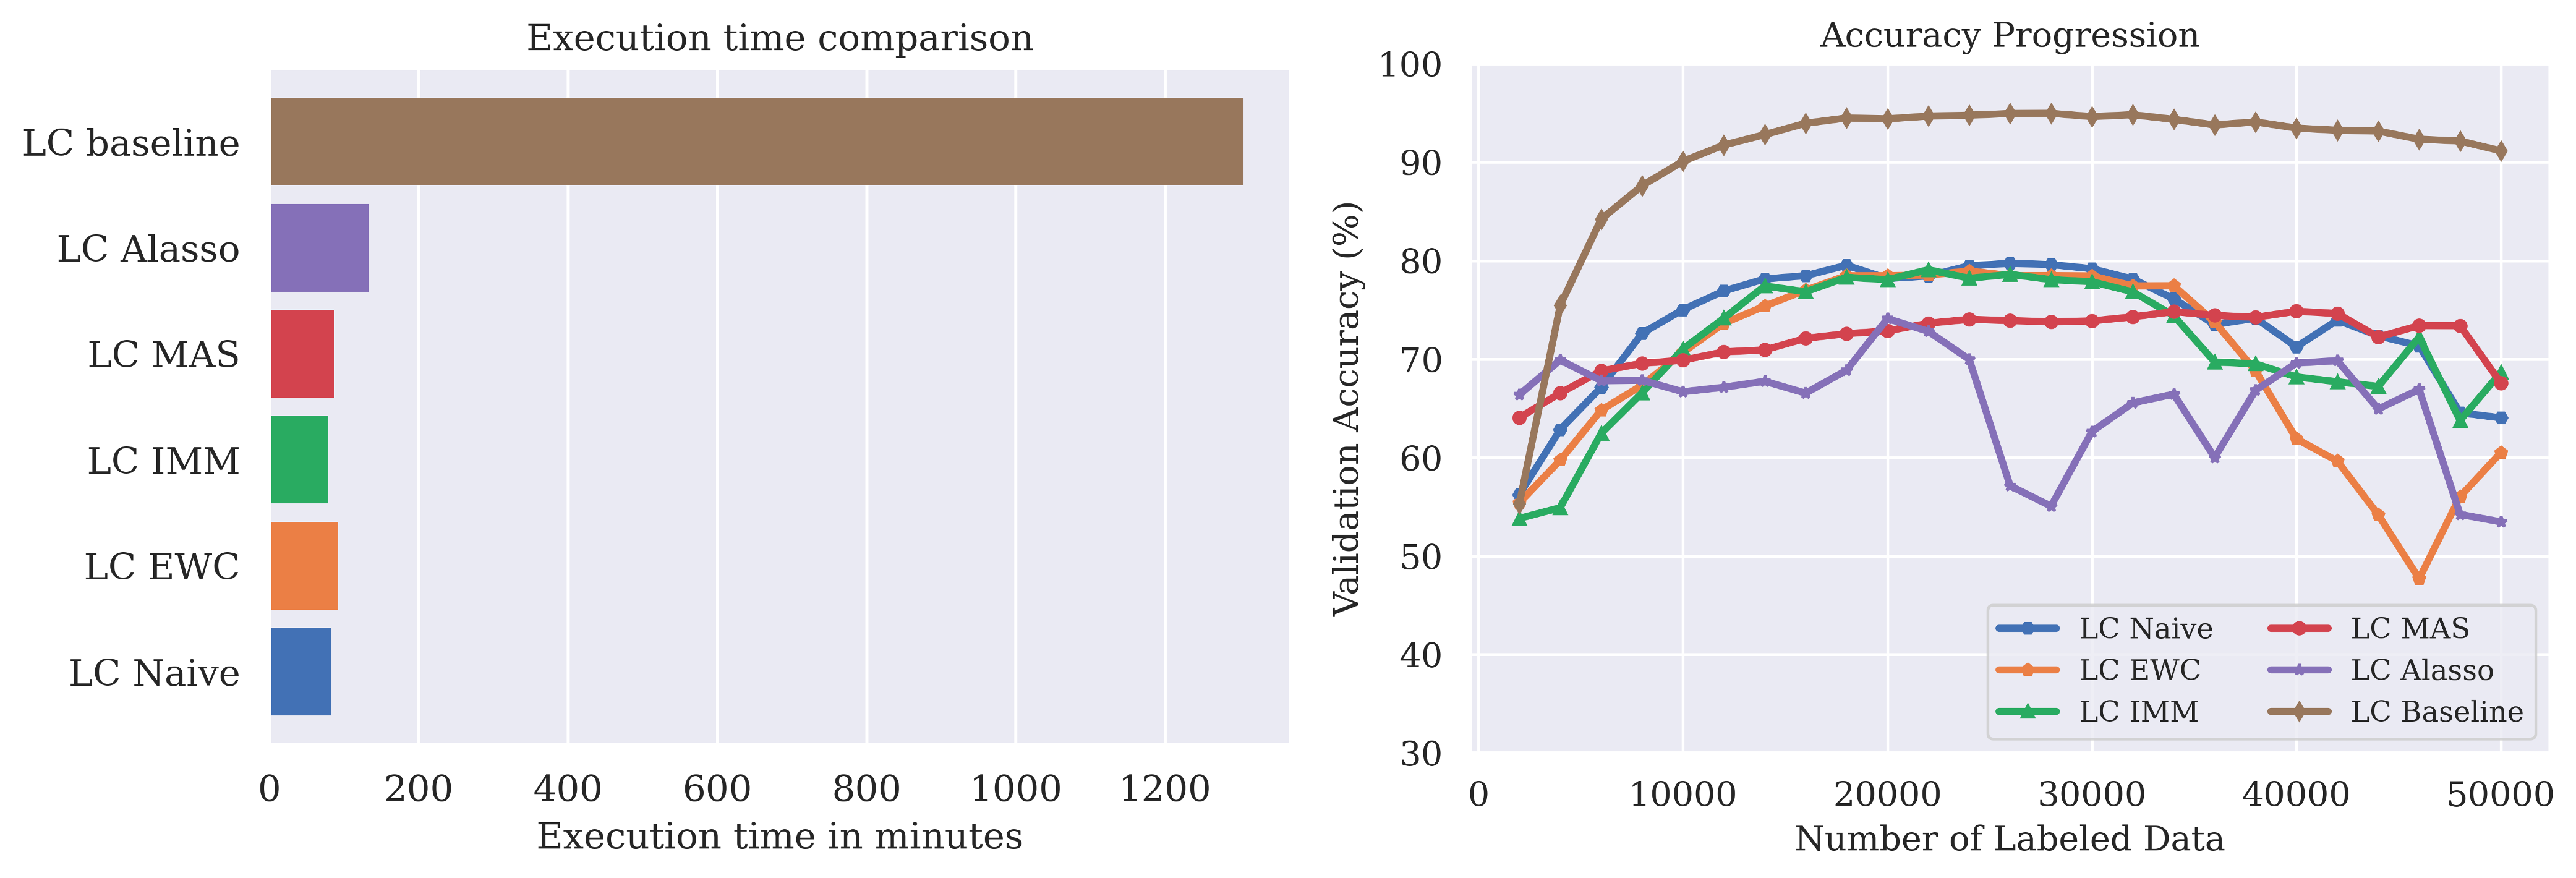
\includegraphics[width=\linewidth]{images/results_CAL/LC_CAL_2000b.png}
    \caption[Continual Active Learning Random 2000 batch size]{Comparison of Continual Learning strategies used with the Active Learning strategy LC. In terms of runtime, all
    strategies are significantly faster than the classic Active Learning approach. However, there is a notable gap in validation accuracy between Active Learning and all Continual
    Active Learning strategies. EWC, IMM and Naive perform similarly, followed by Alasso and MAS. Apart from MAS, all strategies experience a large drop in accuracy after 30000 samples.}
    \label{fig:Evaluation:Results:CAL:LC2000}
\end{figure}

\begin{figure} [ht]
    \centering
    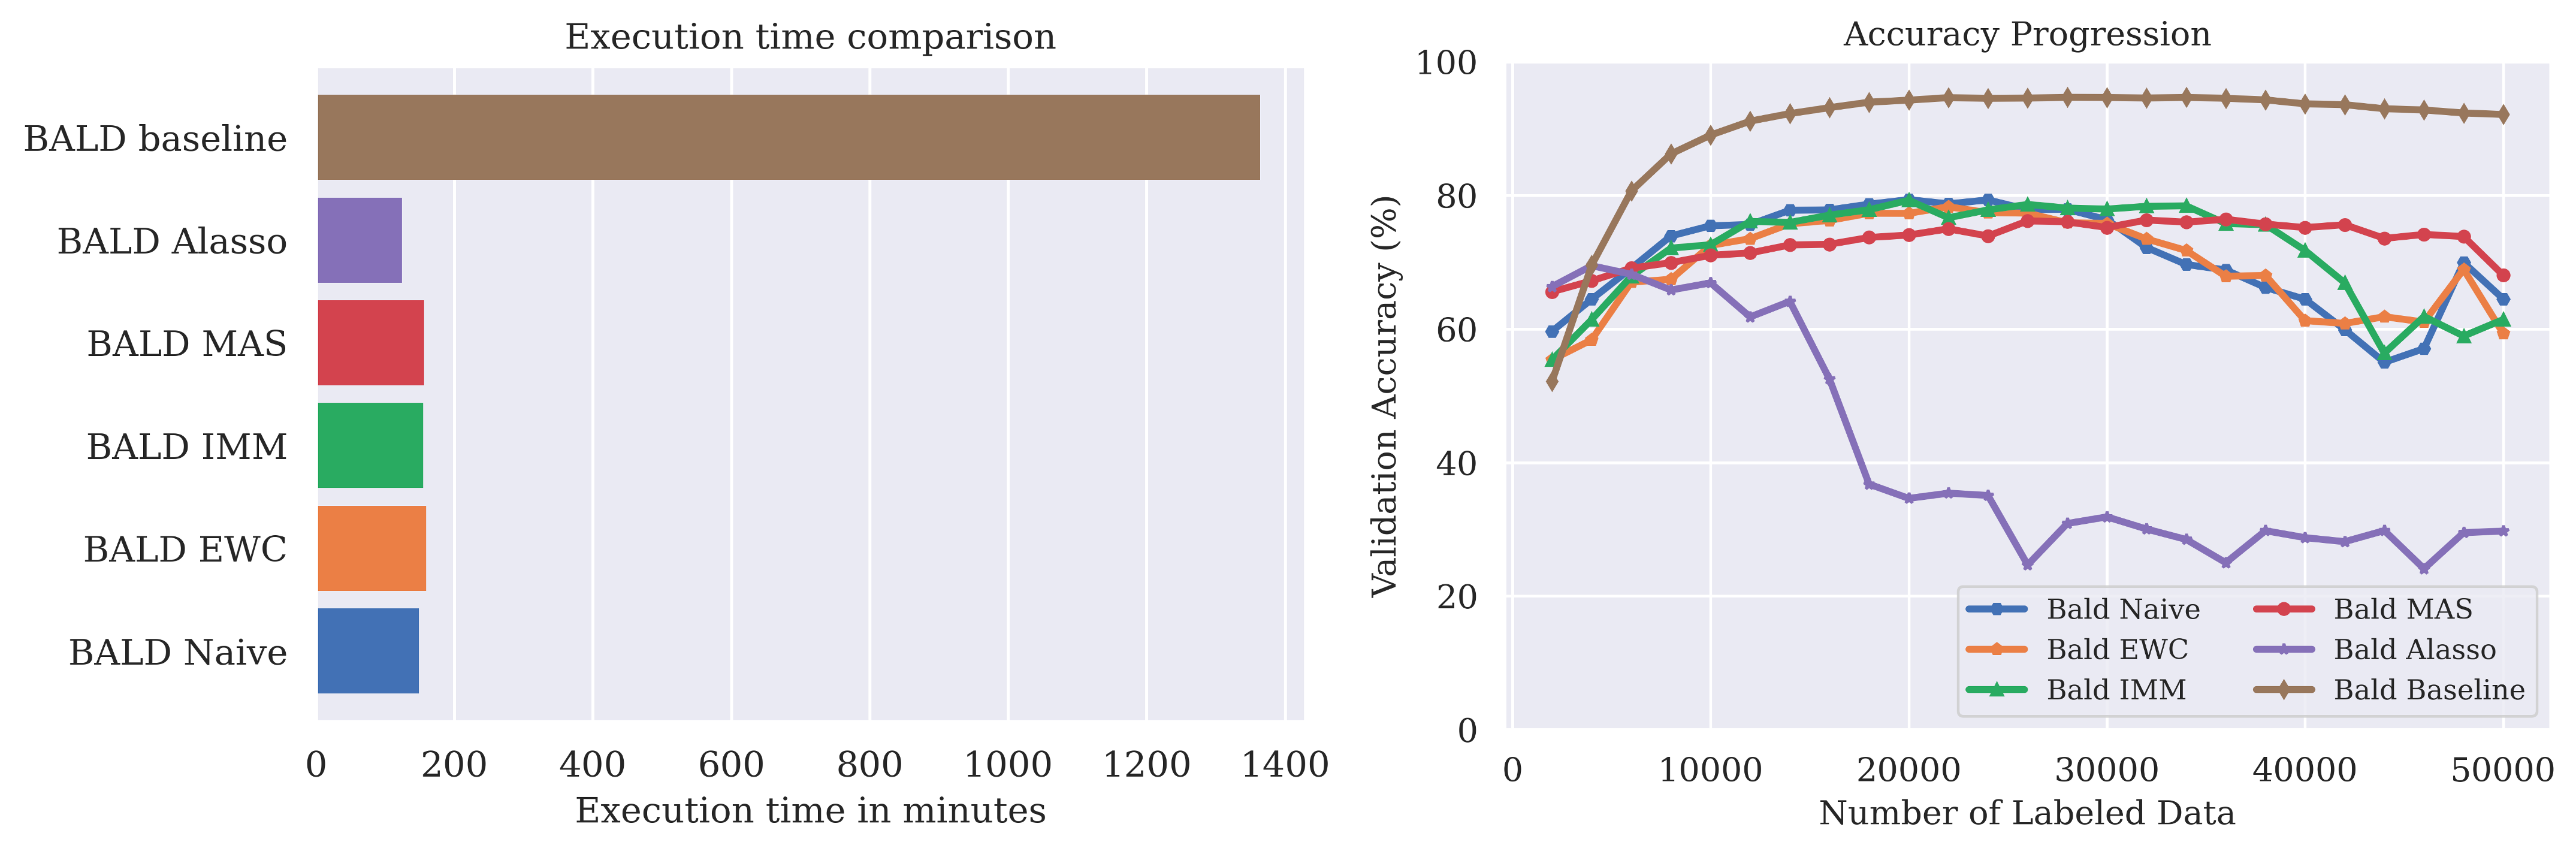
\includegraphics[width=\linewidth]{images/results_CAL/Bald_CAL_2000b.png}
    \caption[Continual Active Learning BALD 2000 batch size]{TODO: Redo BALD plot}
    \label{fig:Evaluation:Results:CAL:BALD2000}
\end{figure}

\begin{figure} [ht]
    \centering
    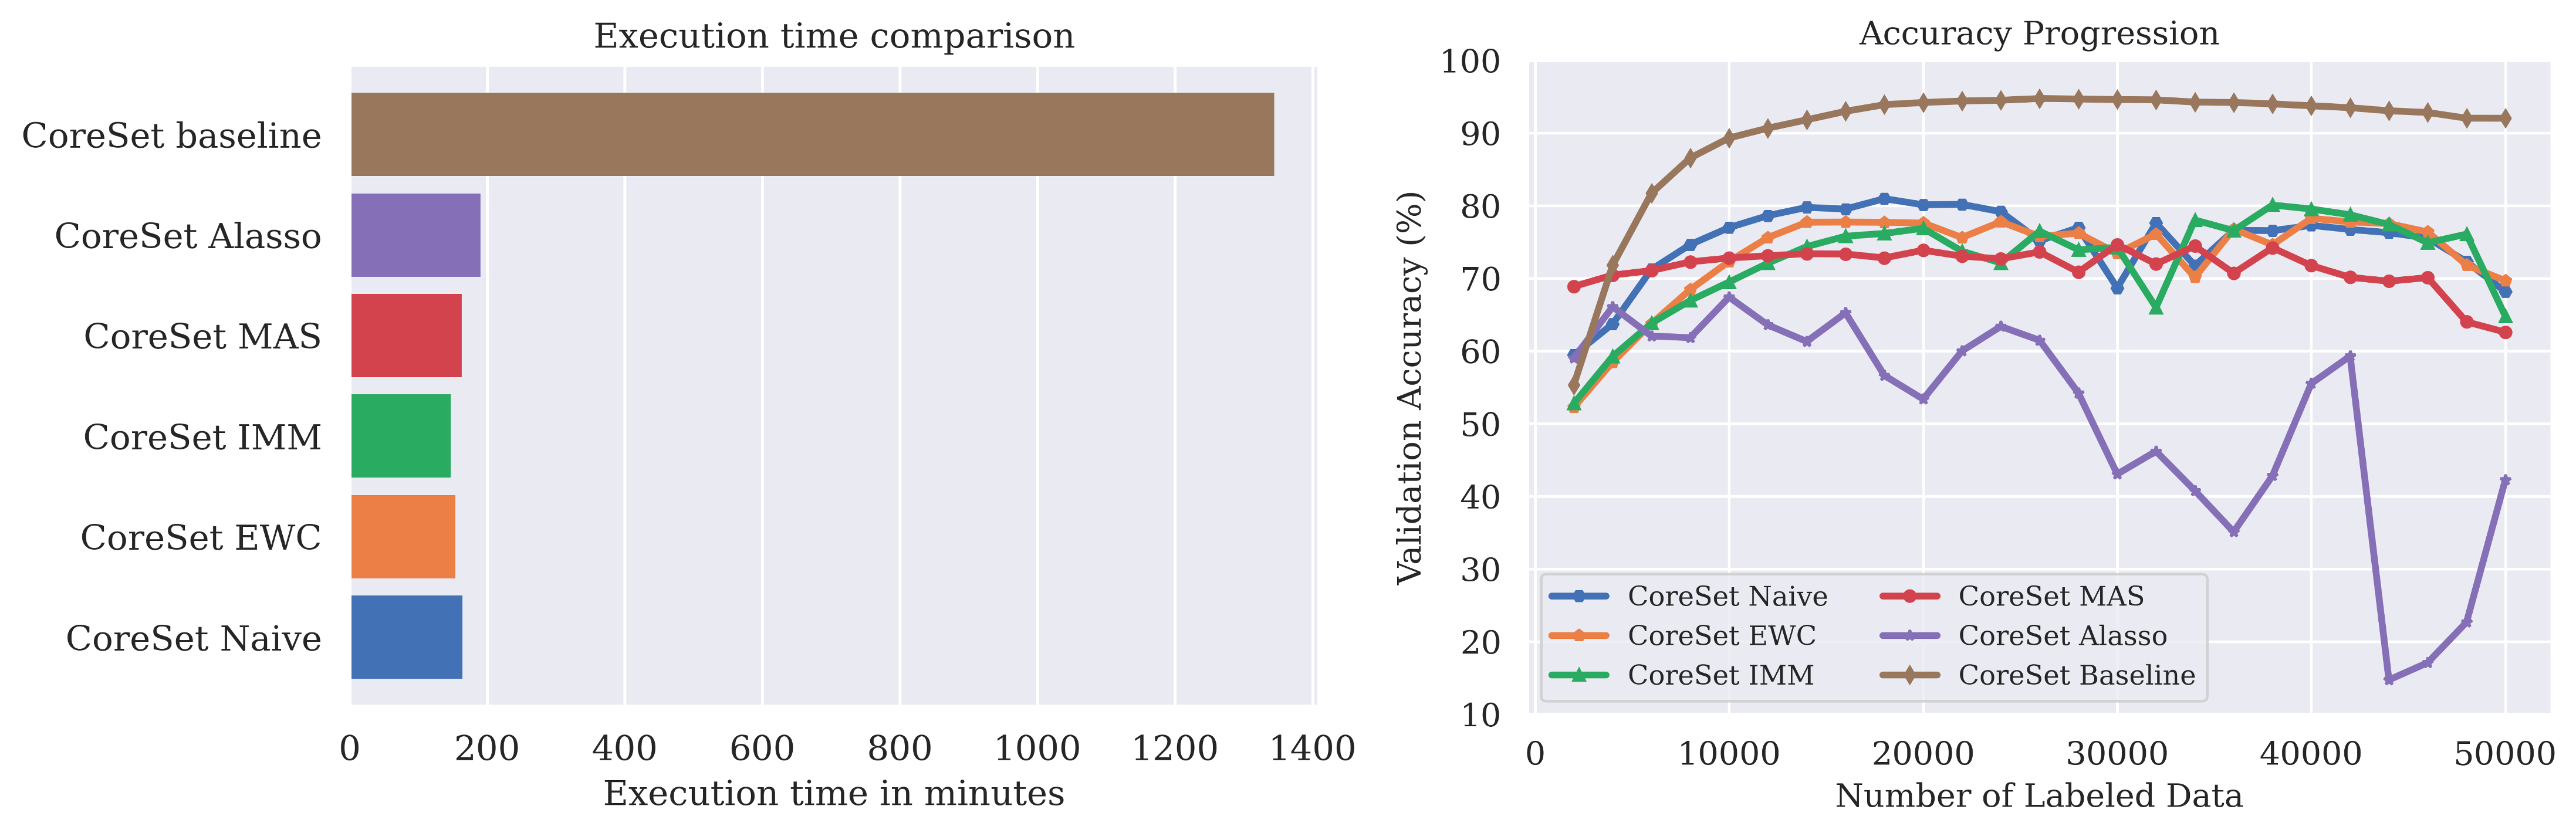
\includegraphics[width=\linewidth]{images/results_CAL/CoreSet_CAL_2000b.png}
    \caption[Continual Active Learning CoreSet 2000 batch size]{Comparison of Continual Learning strategies used with the Active Learning strategy CoreSet. In terms of runtime, all
    strategies are significantly faster than the classic Active Learning approach. However, there is a notable gap in validation accuracy between Active Learning and all Continual
    Active Learning strategies. The Naive approach performs outperforms all other strategies in the first half, but is itself outperformed by IMM and EWC in the second half. MAS performs
    worse than the first three strategies but better than Alasso. The validation accuracy of Alasso becomes worse over time and is significantly worse than the other strategies.}
    \label{fig:Evaluation:Results:CAL:CoreSet2000}
\end{figure}

\begin{figure} [ht]
    \centering
    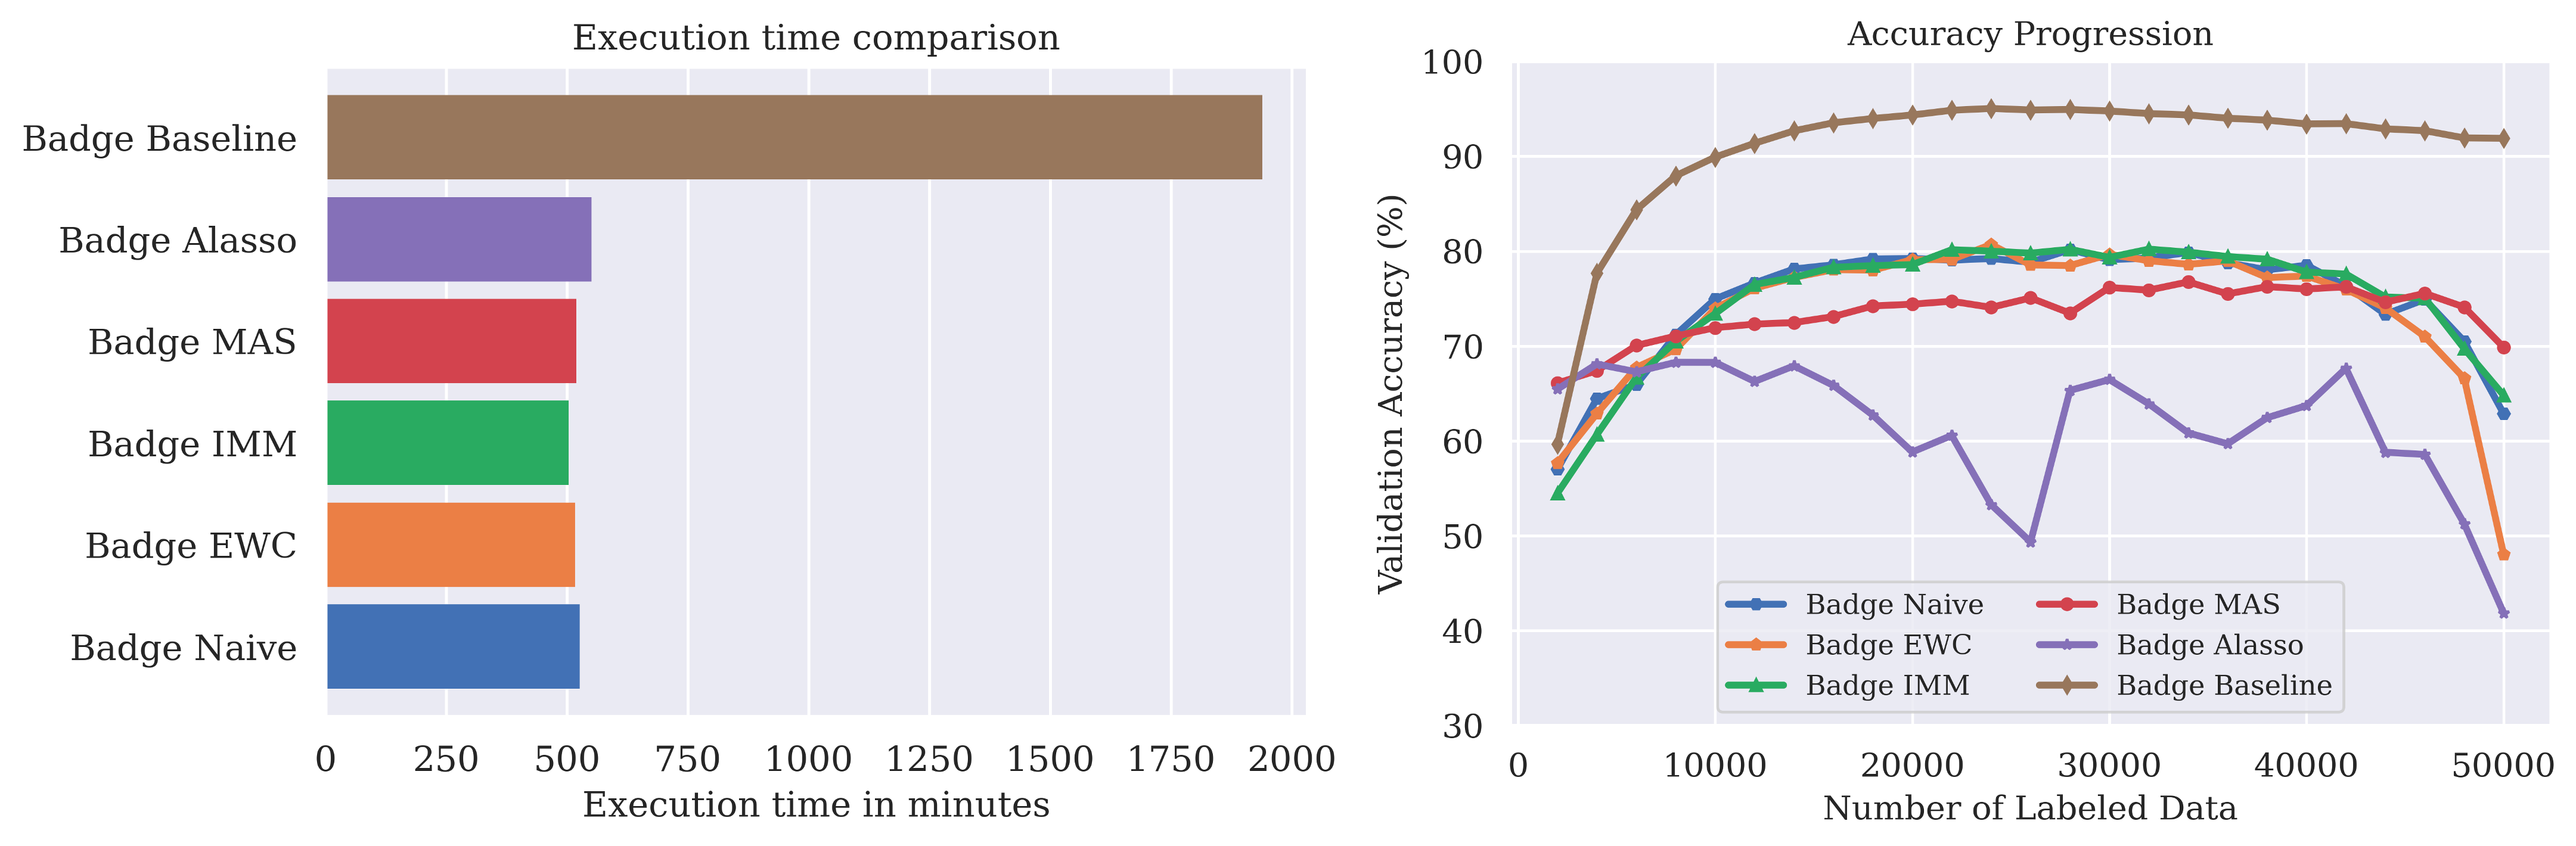
\includegraphics[width=\linewidth]{images/results_CAL/Badge_CAL_2000b.png}
    \caption[Continual Active Learning Badge 2000 batch size]{Comparison of Continual Learning strategies used with the Active Learning strategy Badge. In terms of runtime, all
    strategies are 2.5-3 times faster than the classic Active Learning approach. However, there is a notable gap in validation accuracy between Active Learning and all Continual
    Active Learning strategies. The performance of IMM and EWC is similar to the Naive approach. MAS performs slightly worse than the first three, but 
    worse than the first three strategies but better than Alasso. The validation accuracy of Alasso becomes worse over time and is significantly worse than the other strategies.}
    \label{fig:Evaluation:Results:CAL:Badge2000}
\end{figure}





\begin{figure} [ht]
    \centering
    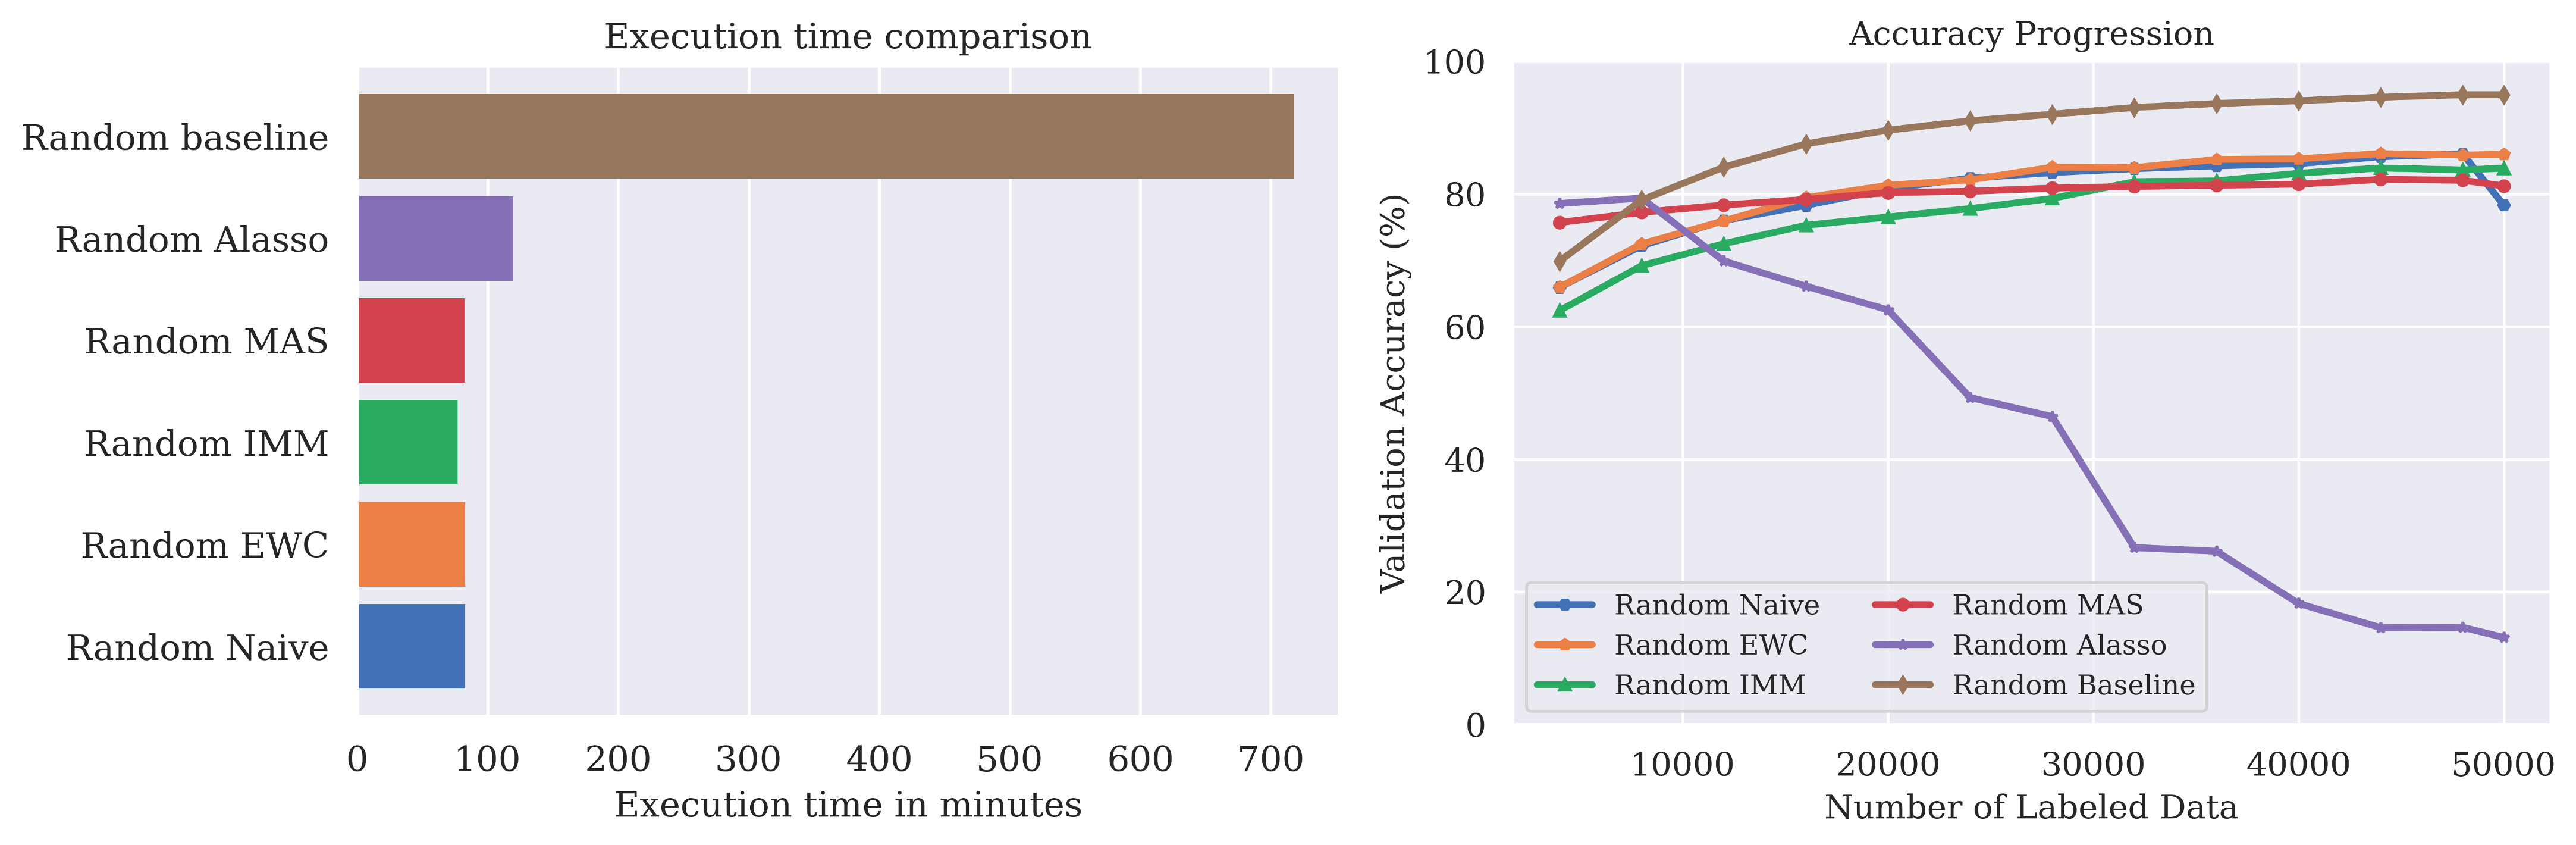
\includegraphics[width=\linewidth]{images/results_CAL/Random_CAL_4000b.png}
    \caption[Continual Active Learning Random 4000 batch size]{Comparison of Continual Learning strategies used with the Active Learning strategy random. In terms of runtime, all
    strategies are 5-9 times faster than the classic Active Learning approach. There is a gap in validation accuracy between Active Learning and all Continual
    Active Learning strategies, however this is lower than the gap for smaller batch sizes. EWC and the Naive approach perform similarly across the whole experiment. MAS and IMM
    also perform similarly overall, however MAS performs better in the first half wheres IMM performs better in the second half. Alasso is the best strategy in the beginning but 
    becomes worse as the number of labeled data increases.}
    \label{fig:Evaluation:Results:CAL:Random4000}
\end{figure}

\begin{figure} [ht]
    \centering
    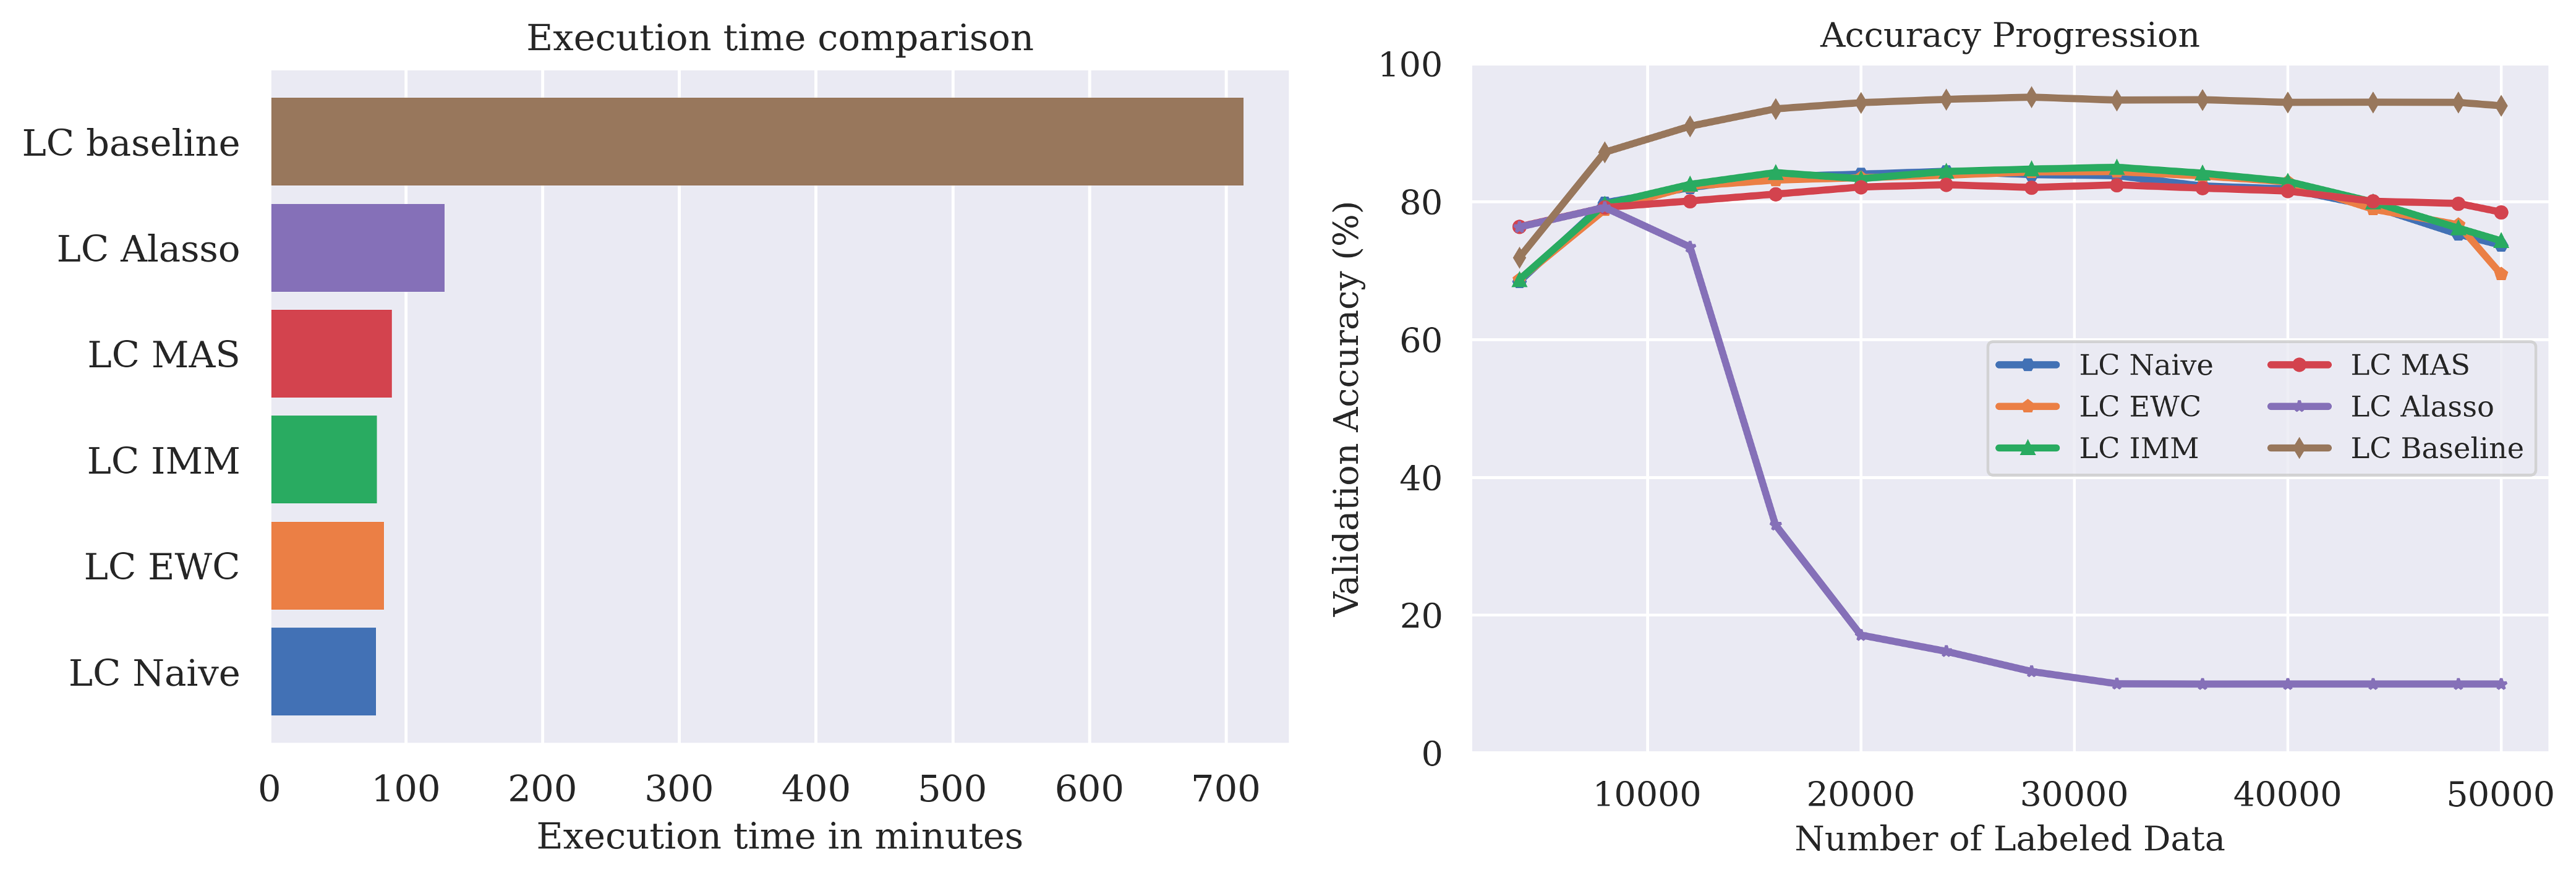
\includegraphics[width=\linewidth]{images/results_CAL/LC_CAL_4000b.png}
    \caption[Continual Active Learning Random 4000 batch size]{Comparison of Continual Learning strategies used with the Active Learning strategy LC. In terms of runtime, all
    strategies are 5-9 times faster than the classic Active Learning approach. There is a gap in validation accuracy between Active Learning and all Continual
    Active Learning strategies, however this is lower than the gap for smaller batch sizes. IMM and EWC perform best, followed by the Naive approach and MAS. Alasso falls behind
    significantly.}
    \label{fig:Evaluation:Results:CAL:LC4000}
\end{figure}

\begin{figure} [ht]
    \centering
    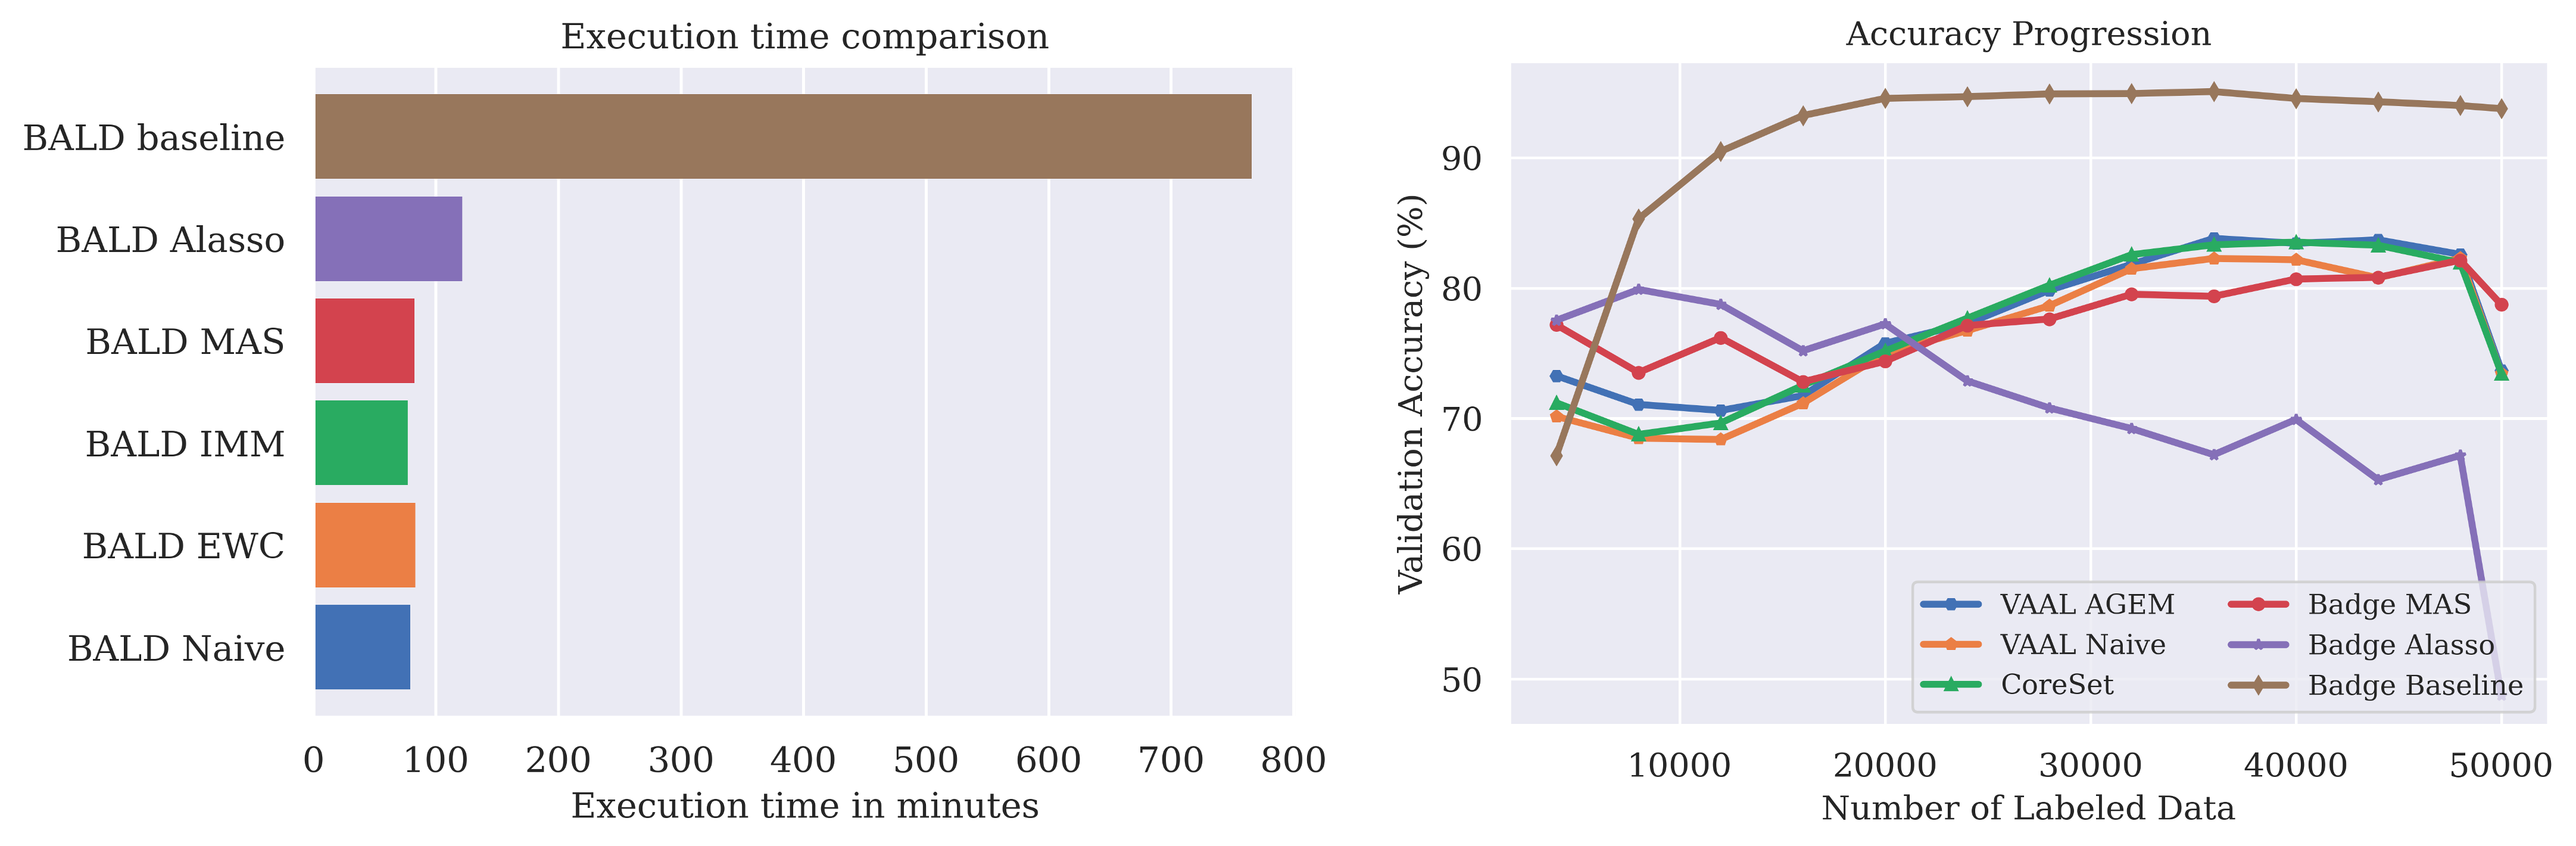
\includegraphics[width=\linewidth]{images/results_CAL/Bald_CAL_4000b.png}
    \caption[Continual Active Learning BALD 4000 batch size]{TODO: Redo BALD plot}
    \label{fig:Evaluation:Results:CAL:BALD4000}
\end{figure}

\begin{figure} [ht]
    \centering
    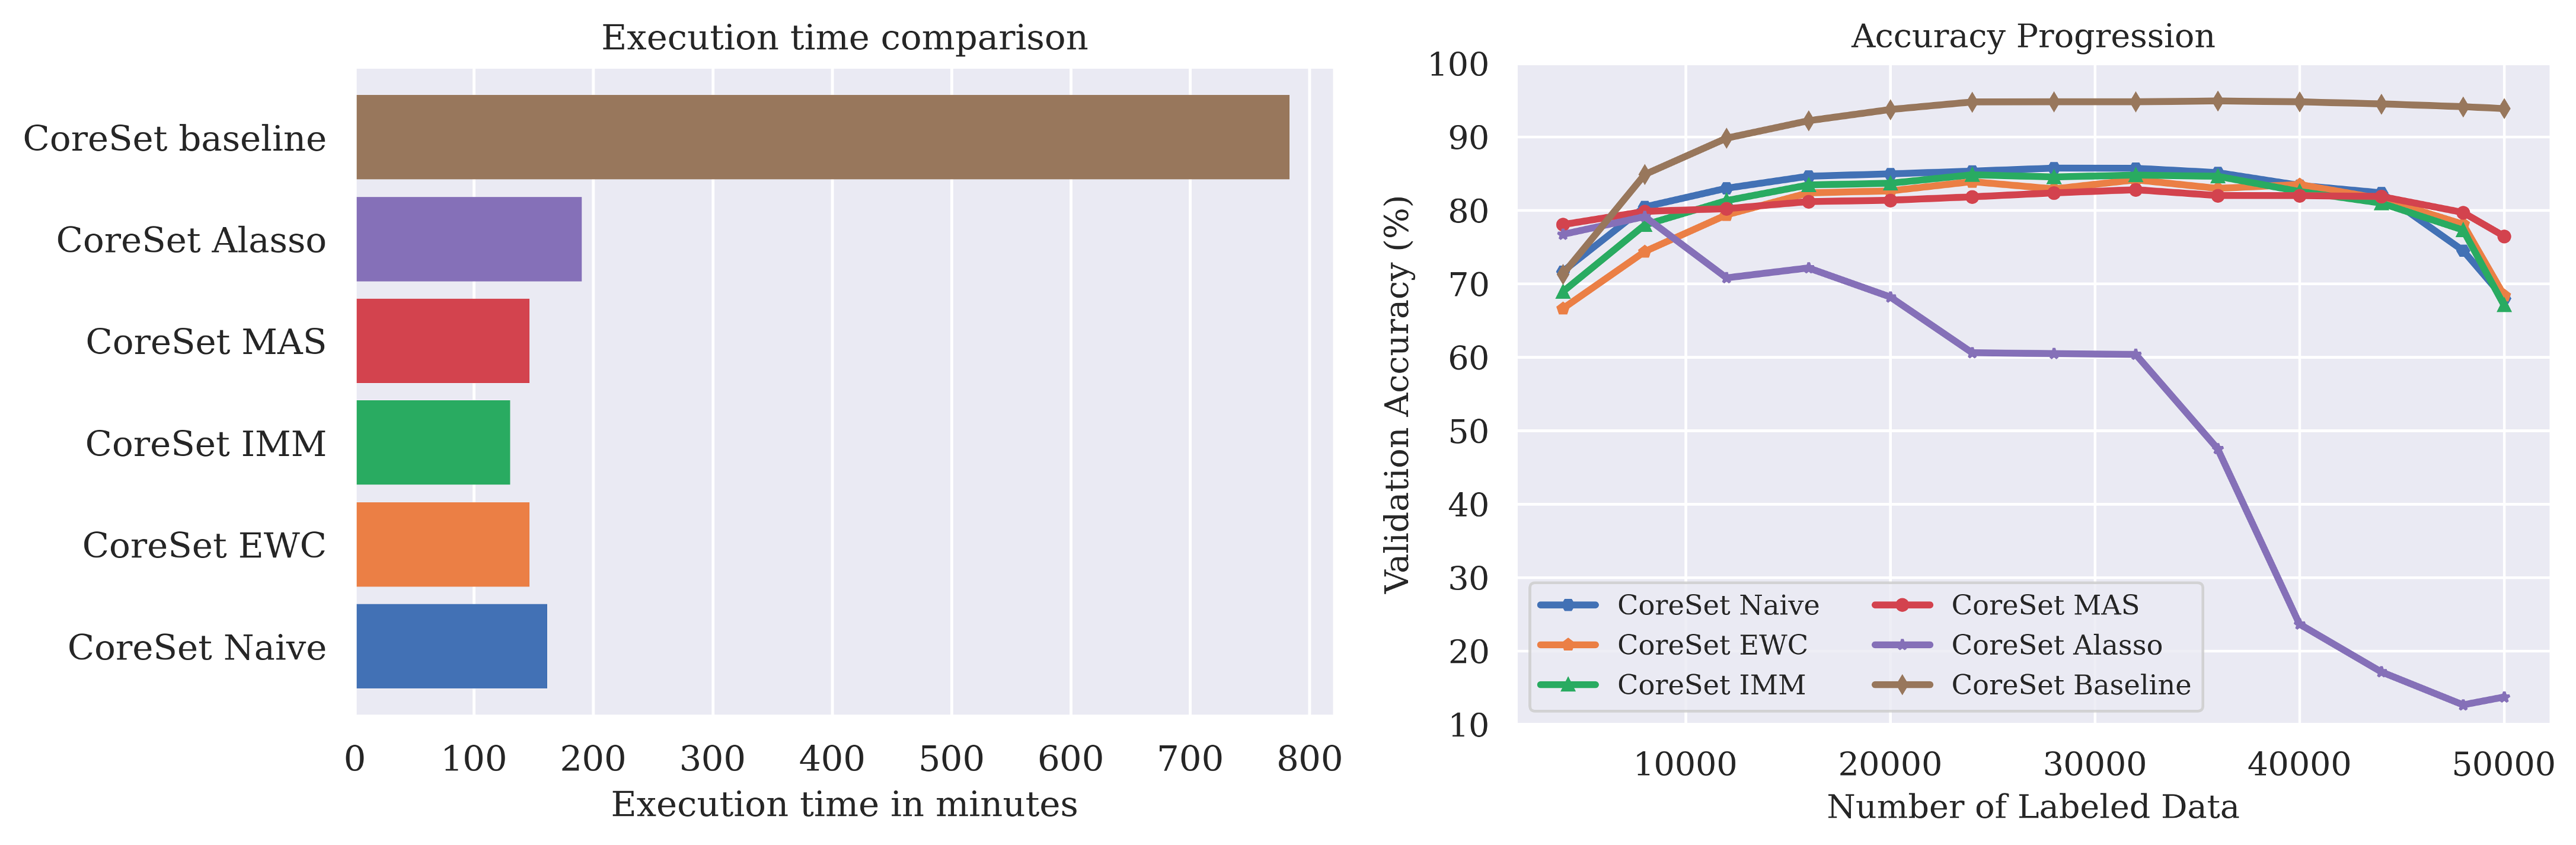
\includegraphics[width=\linewidth]{images/results_CAL/CoreSet_CAL_4000b.png}
    \caption[Continual Active Learning CoreSet 4000 batch size]{Comparison of Continual Learning strategies used with the Active Learning strategy CoreSet. In terms of runtime, all
    strategies are 4-5 times faster than the classic Active Learning approach. There is a gap in validation accuracy between Active Learning and all Continual
    Active Learning strategies, however this is lower than the gap for smaller batch sizes. The Naive approach performs best, followed by IMM, EWC and MAS in this order. The performance
    of Alasso deteriorates over time and falls significantly behind the performance of the remaining approaches.}
    \label{fig:Evaluation:Results:CAL:CoreSet4000}
\end{figure}

\begin{figure} [ht]
    \centering
    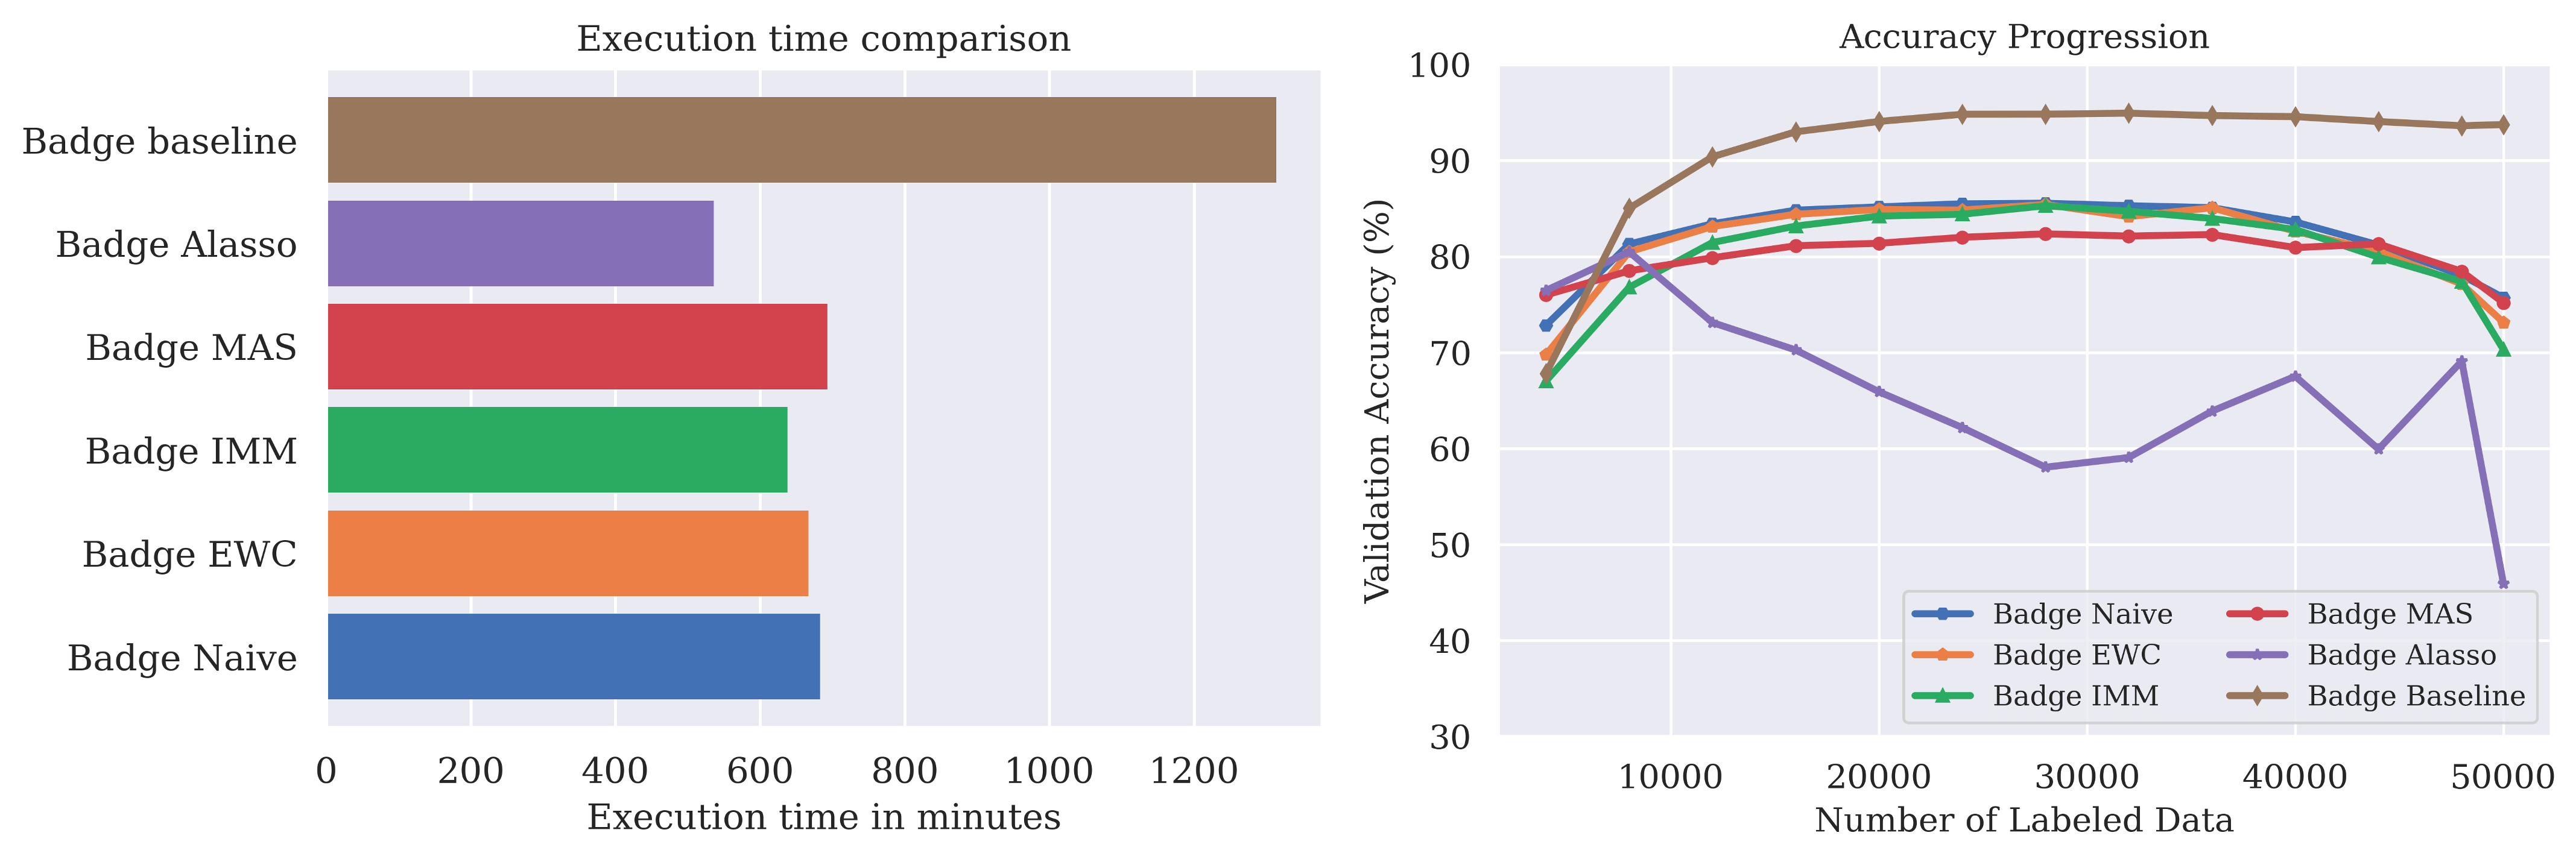
\includegraphics[width=\linewidth]{images/results_CAL/Badge_CAL_4000b.png}
    \caption[Continual Active Learning Badge 4000 batch size]{Comparison of Continual Learning strategies used with the Active Learning strategy Badge. In terms of runtime, all
    strategies are approximately 2 times faster than the classic Active Learning approach. There is a gap in validation accuracy between Active Learning and all Continual
    Active Learning strategies, however this is lower than the gap for smaller batch sizes. The Naive approach performs best, closely followed by EWC. IMM comes third decreasing the
    performance gap to the third two approaches with increasing number of labeled data. MAS follows IMM and Alasso falls behind significantly.}
    \label{fig:Evaluation:Results:CAL:Badge4000}
\end{figure}


\begin{figure} [ht]
    \centering
    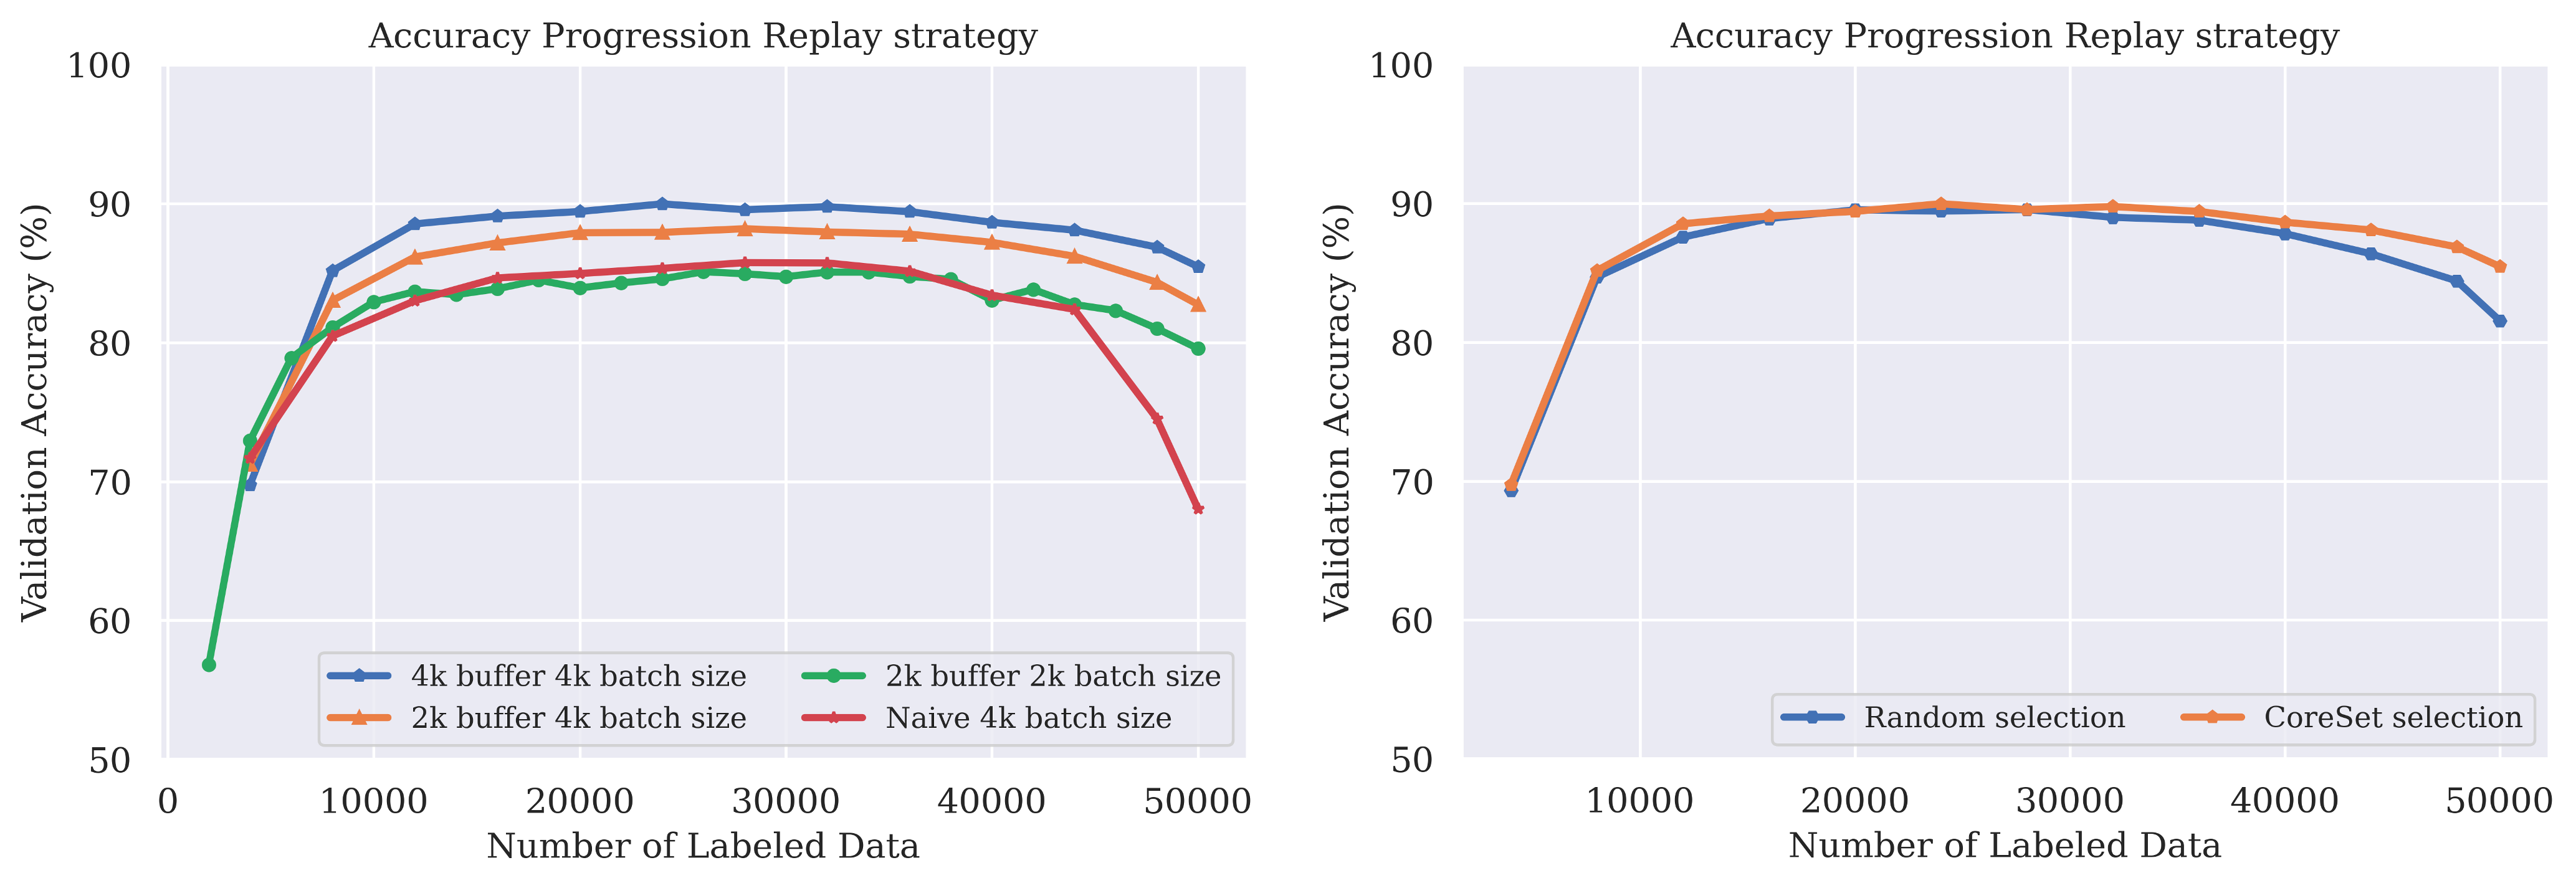
\includegraphics[width=\linewidth]{images/results_CAL/replay_CAL.png}
    \caption[Continual Active Learning Badge 4000 batch size]{TODO: Redo plot}
    \label{fig:Evaluation:Results:CAL:Replay}
\end{figure}

\begin{figure}[ht]
    \centering
    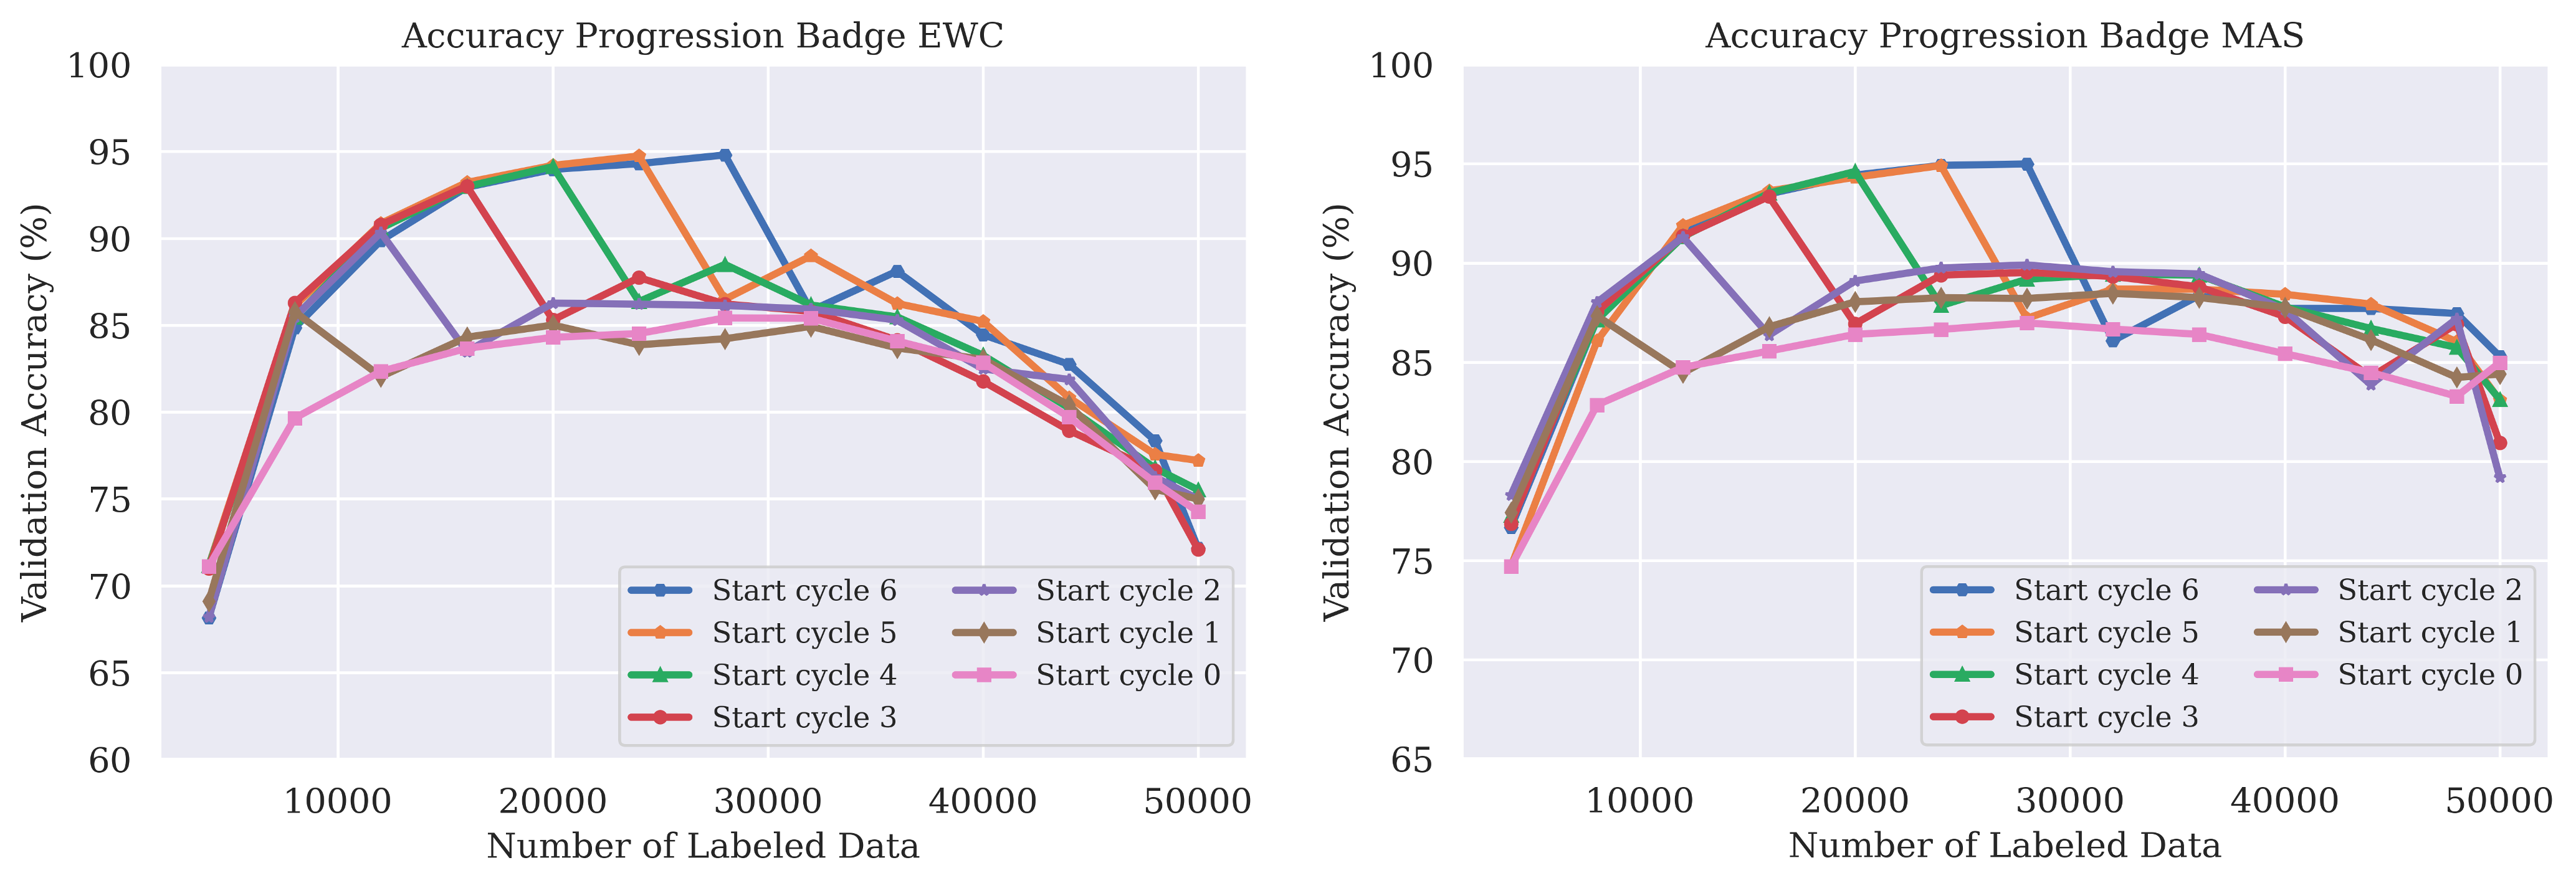
\includegraphics[width=\linewidth]{images/results_CAL/Delayed_start_CAL.png}
    \caption[Continual Active Learning Badge 4000 batch size]{Comparison of validation accuracy for a delayed start of Continual Learning. We vary the start of Continual Learning from 
    cycle 0 (random initialization) to cycle 6, hoping that the model retains the accuracy obtained by training using Active Learning. However, the accuracy drops immediately after switching
    from Active Learning to Continual Active Learning and continues to decrease after 25000 points. While the validation accuracy drops when using both MAS and EWC, MAS does retain the accuracy
    better than EWC.}
    \label{fig:Evaluation:Results:CAL:DelayedStart}
\end{figure}


\begin{figure}[ht]
    \centering
    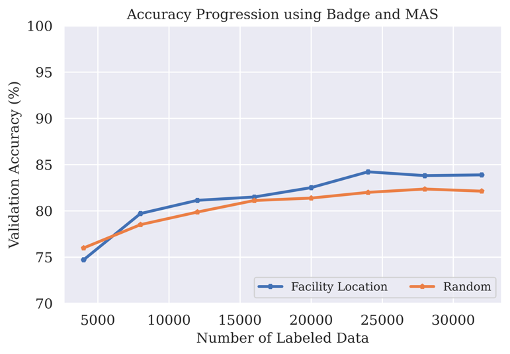
\includegraphics[width=\linewidth]{images/results_CAL/Factility_location_init.png}
    \caption[Initialization using Facility Location]{We try to initialize the labeled pool using Facility Location. Facility location slightly outperforms traditional random initialization, however,
    it achieves a slightly lower validation accuracy in the beginning.}
    \label{fig:Evaluation:Results:CAL:FLinit}
\end{figure}

\subsection{Results for Continual Active Learning for Model Stealing}
\label{sec:Evaluation:Results:CALMS}

\begin{table}
    \centering
    \begin{tabularx}{\textwidth}{l | c c c} 
        \hline
        \diaghead{\theadfont Diag ColumnHead 2}%
        {Target \\ Model}{Substitute \\ Model} &  ActiveThiefConv2 & ActiveThiefConv3 & ActiveThiefConv4 \\ 
        \hline 
        ActiveThiefConv2 & A & B & C \\
        ActiveThiefConv3 & A & B & C \\
        ActiveThiefConv4 & A & B & C \\
        \hline
    \end{tabularx}
    \caption{Success of Model Stealing Attacks for Different NN Architectures on CIFAR-10}
    \label{fig:ModelStealingNNArchitecturesCIFAR}
\end{table}


\begin{table}
    \centering
    \begin{tabularx}{\textwidth}{l | c c c} 
        \hline
        \diaghead{\theadfont Diag ColumnHead 2}%
        {Target \\ Model}{Substitute \\ Model} &  ActiveThiefConv2 & ActiveThiefConv3 & ActiveThiefConv4 \\ 
        \hline 
        ActiveThiefConv2 & A & B & C \\
        ActiveThiefConv3 & A & B & C \\
        ActiveThiefConv4 & A & B & C \\
        \hline
    \end{tabularx}
    \caption{Success of Model Stealing Attacks for Different NN Architectures on MNIST}
    \label{fig:ModelStealingNNArchitecturesMNIST}
\end{table}

\section{Discussion}
\label{sec:Evaluation:ThirdSection}
% Was war das Ziel? Was wurde (nicht) erreicht?

\dots
%% ---------------------
%% | / Example content |
%% ---------------------